%%==================================================================%%
%% Author : Perelló Nieto, Miquel                                   %%
%% Version: 1.0, 04/11/2011                                         %%
%%                                                                  %%
%% Memoria del Projecte de Final de Carrera                         %%
%% Disseny del laboratori                                           %%
%%==================================================================%%

\chapter{Implementació del laboratori}\label{cap:imp}


% the code below specifies where the figures are stored
\ifpdf
    \graphicspath{{4_laboratory_implement/figures/PNG/}{4_laboratory_implement/figures/PDF/}{4_laboratory_implement/figures/}}
\else
    \graphicspath{{4_laboratory_implement/figures/EPS/}{4_laboratory_implement/figures/}}
\fi


% ----------------------- contents from here ------------------------

En aquest apartat aprofundirem en cóm s'ha dut a terme la programació de les diferents parts que conformen el laboratori que hem dissenyat anteriorment (capítol \ref{cap:dis}), i podrem veure d'aquesta manera com podem modificar el codi per ampliar el laboratori amb una infinitud de opcions, modificant o afegint diferents dispositius, o missatges de comunicació.

Per implementar el laboratori hem necessitat crear l'entorn necessari per compartir el bus CAN entre varis llaços de control, i tenir el programa \DCSMonitor connectat al dispositiu \Monitor via RS232, per tant existeix una configuració bàsica formada per dos llaços de control monitoritzats per un dispositiu \Monitor i aquest connectat al programa \DCSMonitor capaç de modificar el comportament d'aquest ultim. Es pot veure una fotografia de tot l'entorn preparat i configurat per tal de treballar amb aquest sistema, i amb el qual s'ha pogut dur a terme tota la fase de implementació (figura \ref{workspace}).

\figuremacro{workspace}{Entorn de treball}{Tot el material necessari per implementar el laboratori amb dos llaços de control, un programador Mplab ICD2, un conversor de RS232 a USB, el programa \DCSMonitor en marxa al monitor esquerra i codi font al monitor de la dreta.}

Hem dividit el capítol en dues seccions principals, la part de programació en \Python del programa \DCSMonitor (el programa que s'executa en l'ordinador) on podrem veure els passos que s'han seguit per crear la interfície visual (secció \ref{cap:imp:visual}), com hem pogut obrir el port RS232 i posteriorment enviar i rebre tot tipus de missatges (secció \ref{cap:imp:com:serie}), com hem integrat els plots del llaç de control que estiguéssim monitoritzant o  connectats (secció \ref{cap:imp:gen:graph}), com hem fet per exportar una gràfica generada en diferents formats (seccio \ref{cap:imp:exp:graph}), com hem realitzat l'actualització de les estadístiques en temps real (secció \ref{cap:imp:estat}), i finalment quins són els passos seguits per implementar els diferents idiomes, i per afegir-ne de nous (secció \ref{cap:imp:idi}). 

I la part de programació en \C en el Sistema Operatiu en Temps Real Erika Enterprise que corre en els diferents dispositius del control (microcontroladors dsPIC33FJ256MC710, en la placa \FLEX), on es podrà veure com implementar noves tasques en el SO Erika (secció \ref{lab:imp:dspic:monitor:tasks}), com hem implementat la recepció i enviament dels diferents missatges per RS232 (secció \ref{cap:imp:com:serie}), i el més important en els sistemes distribuïts la comunicació mitjançant el bus CAN (secció \ref{lab:imp:dspic:can}); la creació de màscares i filtres, la recepció dels diferents missatges, l'enviament d'aquests, i la creació de una pila per mantenir un llistat de tots els llaços de control presents al bus.

\FloatBarrier

\section{\DCSMonitor}\label{cap:imp:dcs}

Com hem vist anteriorment, el programa \DCSMonitor és l'encarregat de mostrar-nos en temps real el funcionament dels diferents controls als que estem connectats via RS232.
Gracies a ell podem monitoritzar un bus CAN (si estem connectats a un dispositiu \Monitor), o podem comprovar que el control que estem executant sigui correcte (connectats directament a un dispositiu \SensorActuador).
En aquest apartat s'explica com s'han programat totes les parts implicades del laboratori que formen part del programa \DCSMonitor, començant per l'aspecte visual, passant per les comunicacions i el mostreig dels plots, i acabant finalment per la integració amb varis idiomes.

Cal indicar que per crear les gràfiques en temps real s'ha pres com a exemple el codi de Yassine Benabbas amb Llicencia Creative Commons present en la bibliografia \cite[Creér un graphe dynamique avec PyPlot]{yassine}.

%====================================================================================%
% Interficie
%====================================================================================%
\subsection{Interficie}\label{cap:imp:visual}

Pel disseny de la part visual del programa es va utilitzar la eina \QTCreator, el qual és un IDE per realitzar interfìcies de programes arrossegant i enganxant les diferents parts. Això ens permet guanyar temps en petits programes, i en programes grans és quasi impossible prescindir d'aquesta ajuda.

Un cop hem realitzat la organització de tots els botons i etiquetes que formen el programa, li indiquem a \QTCreator que ens generi el codi font d'aquest en format \textit{.ui} (es posa un fragment de codi com a exemple, \ref{lab:imp:dsc:interficie:ui}, ja que el codi complert ocupa unes 700 línies, més o menys 25 pàgines)

\begin{code_xml}{Fragment del fitxer d'interficie dcsmmainwindow.ui}{lab:imp:dsc:interficie:ui}
<?xml version="1.0" encoding="UTF-8"?>
<ui version="4.0">
 <class>MainWindow</class>
 <widget class="QMainWindow" name="MainWindow">
  <property name="geometry">
   <rect>
    <x>0</x>
    <y>0</y>
    <width>752</width>
    <height>790</height>
   </rect>
  </property>
  <property name="windowTitle">
   <string>Distributed Control Systems Monitor</string>
  </property>
     ...
\end{code_xml}

Un cop hem generat aquest fitxer és hora de traduir-ho a \Python, per tal de que la llibrería que utilitzem \PyQT pugui generar l'interficie. Per fer aixó ens ajudem del programa \pyuic que amb la comanda \ref{lab:imp:pyuic4} genera un fitxer com el del fragment \ref{lab:imp:interficie:py}

\begin{code_bash}{Creant fitxer d'interficie}{lab:imp:pyuic4}
pyuic4 dcsmmainwindow.ui > dcsmmainwindow.py
\end{code_bash}

\begin{code_python}{Fragment de codi del fitxer dcsmmainwindow.py}{lab:imp:interficie:py}
try:
    _fromUtf8 = QtCore.QString.fromUtf8
except AttributeError:
    _fromUtf8 = lambda s: s

class Ui_MainWindow(object):
    def setupUi(self, MainWindow):
        MainWindow.setObjectName(_fromUtf8("MainWindow"))
        MainWindow.resize(752, 790)
        self.centralwidget = QtGui.QWidget(MainWindow)
\end{code_python}

Finalment es pot veure a la figura \ref{exemple_saturat_03} el resultat d'aquests passos, amb una captura de la pantalla de l'execució.
\begin{landscape}
\figuremacroW{exemple_saturat_03}{Interfície final del programa \DCSMonitor}{Captura de pantalla del programa \DCSMonitor mostrant el control amb el bus CAN saturat al 89\%, sense el plot de la primera integral i en anglès.}{1.4}
\end{landscape}

\FloatBarrier

%====================================================================================%
% Comunicació sèrie RS232
%====================================================================================%
\subsection{Comunicació sèrie RS232}\label{cap:imp:com:serie}

Ja hem vist en la secció de disseny dels tipus de missatge serie \ref{cap:dis:comSer} els diferents missatges que han de enviar-se entre el programa \DCSMonitor i els dispositius, ara veurem com hem implementat aquest tipus de comunicacions per la part de l'ordinador.

En aquest apartat indicarem com hem fet per configurar el port serie amb \PySerial, els mètodes que hem utilitzat per enviar els senyals al dispositiu connectat, i com hem rebut els valors necessaris per poder mostrar les gràfiques o llistar els diferents llaços del bus CAN.

%====================================================================================%
% Obrinr dispositiu
%====================================================================================%
\subsubsection{Obrir i tancar dispositiu sèrie}\label{cap:imp:com:serie:openclose}

Per utilitzar aquest tipus de comunicació primer de tot hem de decidir alguns dels paràmetres que porta associats el tipus de comunicació serie. Com anteriorment en el laboratori ja es van ajustar aquests paràmetres el que farem és adaptar-nos a ells i configurar el dispositiu tal i com estava funcionant.

Per fer això primer de tot importem el paquet serial de \Python, i tot seguit assignem els valors als diferents paràmetres (codi \ref{cap:imp:com:serie:conf:code}).

\begin{code_python}{Codi per configurar dispositiu sèrie}{cap:imp:com:serie:conf:code}
# for communicate with pic
import serial

PORT = '/dev/ttyUSB0'
BAUDRATE = 115200
BYTESIZE = serial.EIGHTBITS
PARITY = serial.PARITY_NONE
STOPBITS = serial.STOPBITS_ONE
TIMEOUT = 10
\end{code_python}

Amb tots els paràmetres ben instanciats, ja podem esperar el senyal de connexió per activar aquest dispositiu. El metode que s'utilitza és mitjançant un botó a la interfície del programa, la qual està enllaçada amb un senyal.
En el moment en el que el botó sigui premut, s'activarà la funció que li hem indicat (codi \ref{cap:imp:com:serie:openclose:trig:code}).

\begin{code_python}{Disparador de connexió de port serie}{cap:imp:com:serie:openclose:trig:code}
QtCore.QObject.connect(self.pushButton_connect, QtCore.SIGNAL("clicked()"), self.clicked_connect)
\end{code_python}

La funció amb la que està enllaçada el botó comprovarà si s'està activant o s'està desactivant. Si es prem per activar el dispositiu, provarà d'activar el port serie cridant a la funció \emph{connect\_serial} (codi \ref{cap:imp:com:serie:openclose:connect:code}, explicat més endavant), si això te èxit habilitarà tots els botons que estiguin permesos segons el mode d'execució en el que es trobi el programa (PC$->$\SensorActuador o PC$->$\Monitor) (figura \ref{serie_connectat}), en cas contrari marcarà en vermell que no s'ha pogut connectar (figura \ref{serie_error}).

En el cas en que s'estigui desconnectant el dispositiu serie, aturarà tots els events periòdics que estiguin activats (recepció de dades, dibuix de la gràfica i calcul d'estadístiques), tanca el dispositiu serie, i finalment desactivarà tots els botons que no calen usar.

\begin{code_python}{Codi per obrir/tancar dispositiu sèrie}{cap:imp:com:serie:openclose:buton:code}
def clicked_connect(self):
	if not self.pushButton_connect.isChecked():
		self.timer_graph.stop()
		self.timer_data.stop()
		self.timer_statistics.stop()
		self.ser.close()
		self.ser = 0
		self.lineEdit_state.setPalette(QtGui.QPalette(QtGui.QColor("gray")))
		self.lineEdit_state.setText(QtGui.QApplication.translate("MainWindow", "Disconnected", None, QtGui.QApplication.UnicodeUTF8))
		self.pushButton_connect.setText(QtGui.QApplication.translate("MainWindow", "Connect", None, QtGui.QApplication.UnicodeUTF8))
		self.pushButton_monitor.setEnabled(0)
		self.pushButton_monitor.setChecked(0)
		self.pushButton_reload.setEnabled(0)
		self.slider_saturation.setEnabled(0)
		
	else:
		if self.connect_serial():
		    self.lineEdit_state.setPalette(QtGui.QPalette(QtGui.QColor("green")))
		    self.lineEdit_state.setText(QtGui.QApplication.translate("MainWindow", "Connected", None, QtGui.QApplication.UnicodeUTF8))
		    self.pushButton_connect.setText(QtGui.QApplication.translate("MainWindow", "Disconnect", None, QtGui.QApplication.UnicodeUTF8))
		    self.pushButton_monitor.setEnabled(1)
		    self.slider_saturation.setEnabled(1)
		    if self.actionPC_Monitor.isChecked():
		        self.pushButton_reload.setEnabled(1)
		else:
		    self.lineEdit_state.setPalette(QtGui.QPalette(QtGui.QColor("red")))
		    self.lineEdit_state.setText(QtGui.QApplication.translate("MainWindow", "Error connecting", None, QtGui.QApplication.UnicodeUTF8))
		    self.pushButton_connect.setChecked(0)
\end{code_python}


La funció \emph{connect\_serial} és l'encarregada de connectar el dispositiu serie, primer de tot comprova si el dispositiu ja havia estat engegat algun cop. Si no ho havia estat li assigna tots els paràmetres anteriorment instanciats, i posteriorment intenta connectar. En cas de error la funció retornarà 0, en cas contrari retornarà 1.
En cas que el dispositiu ja hagués estat obert anteriorment, la configuració ja està instanciada, per tant només provarem d'obrir-la de nou. Igual que abans retornarà zero o u segons hagi fracassat o connectat amb èxit (codi \ref{cap:imp:com:serie:openclose:connect:code}).

\begin{code_python}{Codi per connectar port serie}{cap:imp:com:serie:openclose:connect:code}
def connect_serial(self):
        """Connects to the serial device, if not return 1"""
        if self.ser == 0:
            try:
                self.ser = serial.Serial(PORT, BAUDRATE, BYTESIZE, PARITY, STOPBITS, TIMEOUT)
                #self.ser = serial.Serial('/dev/ttyUSB0', 115200, timeout=10)
            except:
                self.textBrowser.append(QtGui.QApplication.translate("MainWindow", "\n\t----Failed to connect to the device----\n", None, QtGui.QApplication.UnicodeUTF8))
                return 0
        # this code shouldn't be never executed
        else:
            try:
                self.ser.open()
            except:
                self.textBrowser.append(QtGui.QApplication.translate("MainWindow", "\n\t----Failed to connect to the device----\n", None, QtGui.QApplication.UnicodeUTF8))
                return 0
        return 1
\end{code_python}

Tot seguit es pot veure els canvis que s'efectuen durant la connexió del port serie, en la primera imatge abans de connectar al dispositiu \emph{/dev/ttyUSB0}, després un cop ja s'ha establert la connexió, un cop hem desconnectat correctament el port, i la ultima imatge quan hi ha algun problema de connexió (figura \ref{fig:comparacio:rs232}).

\begin{figure}[ht!]
	\subfloat[Pendent de connectar.]{\label{serie_pendent}
		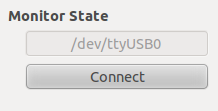
\includegraphics[width=0.25\linewidth]{serie_pendent}
	}
	\subfloat[Connectat correctament.]{\label{serie_connectat}
		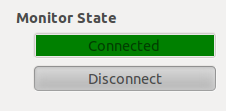
\includegraphics[width=0.25\linewidth]{serie_connectat}
	}
	\subfloat[Desconnectat correctament.]{\label{serie_desconnectat}
		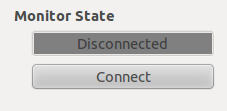
\includegraphics[width=0.25\linewidth]{serie_desconnectat}
	}
	\subfloat[Error al connectar.]{\label{serie_error}
		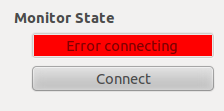
\includegraphics[width=0.25\linewidth]{serie_error}
	}
	\caption{Estat de connexió amb el \Supervisor via RS232.}
    \label{fig:comparacio:rs232}
\end{figure}

\FloatBarrier

%====================================================================================%
% Enviar petició de llistar dispositius
%====================================================================================%
\subsubsection{Enviar petició de llistar llaços de control}\label{cap:imp:com:serie:send:devices}

Al connectar el programa \DCSMonitor amb un dispositiu \Monitor el que ens interessa primer de tot és veure una llista dels diferents llaços de control existents al bus CAN. Aquesta acció només es pot iniciar quan el port serie esta degudament connectat i si el programa s'està executant en mode PC$->$Monitor, per aquest motiu el botó que permet fer aquesta crida romandrà si no es compleixen aquestes dues premisses.

Per activar-ho s'ha creat un disparador que enllaça el botó \emph{Llistar} amb la funció \emph{toogled\_reload} (codi del disparador \ref{cap:imp:com:serie:send:devices:trig:code}).

\begin{code_python}{Disparador de botó llistar dispositius}{cap:imp:com:serie:send:devices:trig:code}
QtCore.QObject.connect(self.pushButton_reload, QtCore.SIGNAL(_fromUtf8("clicked()")), self.toggled_reload)
\end{code_python}

Primer de tot al entrar a aquesta funció (codi \ref{cap:imp:com:serie:send:devices:code})comprova que estem correctament connectats al port serie, si no és així atura aquest procés. Si en canvi tot és correcte, comprova si estem aturant o estem iniciant la recepció d'identificadors, així que segons el que estem realitzant codificarà un o un altre missatge per després enviar-lo pel port serie (les codificacions és poden veure en la figura \ref{fig:bit_encoding:percent} del capítol de disseny)

En el cas de començar a demanar els identificadors, s'activa una alarma periòdica la qual està enllaçada a una funció que captura els missatges que es reben al port serie. Aquesta recepció es pot veure en la secció \ref{cap:imp:com:serie:rec:devices}.
En el cas de aturar aquesta petició, comprovarà si s'està monitoritzant, en cas negatiu aturarà la recepció de dades.

\begin{code_python}{Codi per demanar una llista de llaços de control}{cap:imp:com:serie:send:devices:code}
def toggled_reload(self):
    """Stops or Start to recive devices id's"""
    if not self.connect_serial():
        self.pushButton_reload.setChecked(0)
        return
        
    if self.pushButton_reload.isChecked():
        self.listWidget_link.clear()
        word = struct.pack("BBBBBBBB", ID_DEVICES,0,0,0,0,0,0,0)
        self.timer_data.start(DATA_TIME)
        
    else:
        word = struct.pack("BBBBBBBB", ID_DEVICES + ID_STOP,0,0,0,0,0,0,0)
        if (not self.pushButton_monitor.isChecked()):
            self.timer_data.stop()
        
    self.textBrowser.append(QtGui.QApplication.translate("MainWindow", "Sent : ", None, QtGui.QApplication.UnicodeUTF8)+binascii.hexlify(word)+"\n")
    
    self.ser.write(word)
\end{code_python}




%====================================================================================%
% Enviar petició de monitorització
%====================================================================================%
\subsubsection{Enviar petició de monitorització}\label{cap:imp:com:serie:send:monit}

Aquesta és la acció principal sobre la que es bassa el programa, en el moment que volem veure la gràfica en temps real d'un llaç de control hem d'enviar aquesta petició al \Monitor. Però també podem estar connectats a un dispositiu \SensorActuador, però en aquest cas ; com ja hem explicat en seccions anteriors (secció \ref{diss:nou}); aquesta petició es perdrà, però posarem en marxa tota la part de recepció de dades.

Primer de tot creem el disparador que detectarà que s'ha premut el botó per monitoritzar (codi \ref{cap:imp:com:serie:send:monit:trig:code}), aquest cridarà la funció \emph{toogled\_monitor} (codi \ref{cap:imp:com:serie:send:monit:code}).

\begin{code_python}{Disparador de botó per monitoritzar}{cap:imp:com:serie:send:monit:trig:code}
QtCore.QObject.connect(self.pushButton_monitor, QtCore.SIGNAL("clicked()"), self.toggled_monitor)
\end{code_python}

Aquesta serà la funció detectarà si el que volem és aturar o començar la monitorització, en cas d'iniciar-la comprovarà si hi ha un identificador de llaç de control de la llista seleccionat. Si hi és formarem el missatge amb aquest identificador, en cas contrari monitoritzarem el llaç de control numero u. Tot seguit enviarem aquest senyal per el port serie, netejarem el buffer d'entrada per no confondre algun senyal residual anterior amb un de nou. Netegem la gràfica i activem una funció (\emph{get\_periodical\_data}, veure codi \ref{cap:imp:com:serie:rec:monitor:perio:code}) que rep periòdicament informació per el port serie i la emmagatzema en arrays (els quals ens permetran dibuixar la gràfica), i activa una altre tasca periòdica que en cas de existir dades noves en els arrays tornarà a dibuixar la gràfica (secció de generació de gràfiques en temps real \ref{cap:imp:gen:graph}).
En el cas que estem parant la monitorització aturarem la tasca periòdica que dibuixava la gràfica, i si no s'estan rebent identificadors també aturarem la recepció de dades.

\begin{code_python}{Codi per demanar monitoritzar un llaç de control}{cap:imp:com:serie:send:monit:code}
def toggled_monitor(self):
	"""Starts or Stops reciving data"""
	if self.pushButton_monitor.isChecked():
		
		if not self.connect_serial():
		    self.pushButton_monitor.setChecked(0)
		    return
		
		self.textBrowser.insertPlainText(QtGui.QApplication.translate("MainWindow", "\n\t----NEW MONITORING----\n", None, QtGui.QApplication.UnicodeUTF8))
		
		id_link = self.listWidget_link.selectedItems()
		if len(id_link):
		    id_link = int(id_link[0].text())
		else:
		    id_link = 1
		
		self.textBrowser.insertPlainText(QtGui.QApplication.translate("MainWindow", "link to monitor : ", None, QtGui.QApplication.UnicodeUTF8)+str(id_link)+"\n")
		
		word = struct.pack("BBBBBBBB", ID_MONITOR,0,0,0,0,0,0,id_link&0xFF)

		self.textBrowser.append(QtGui.QApplication.translate("MainWindow", "Sent : ", None, QtGui.QApplication.UnicodeUTF8)+binascii.hexlify(word)+"\n")

		self.ser.write(word)
		 
		# clear data of the serial port
		self.ser.flushInput()
		# clear graph
		self.clean_graph()
		# start timer data reception
		self.get_periodical_data()
		# start timer graphic refresh
		self.update_graph()
		
		self.pushButton_save.setEnabled(False)
	else:
		# send Monitor
		word = struct.pack("BBBBBBBB", ID_MONITOR+ID_STOP,0,0,0,0,0,0,0)

		self.textBrowser.append(QtGui.QApplication.translate("MainWindow", "Sent : ", None, QtGui.QApplication.UnicodeUTF8)+binascii.hexlify(word)+"\n")

		self.ser.write(word)
		
		self.ser.flushInput()
		
		# reload number of waiting chars in serial rx buffer
		self.label_rx_buff_value.setText(str(self.ser.inWaiting()))
		
		self.textBrowser.insertPlainText(QtGui.QApplication.translate("MainWindow", "\n\t----END MONITORING----\n", None, QtGui.QApplication.UnicodeUTF8))
		
		self.pushButton_save.setEnabled(True)
		
		if (not self.pushButton_reload.isChecked()):
		    self.timer_data.stop()
		self.timer_graph.stop()
\end{code_python}


%====================================================================================%
% Enviar percentatge de saturació
%====================================================================================%
\subsubsection{Enviar percentatge de càrrega}\label{cap:imp:com:serie:send:sat}

Igual que en els casos anteriors per enviar aquest missatge al dispositiu \Monitor ho farem a través d'un disparador (codi \ref{cap:imp:com:serie:send:sat:trig:code}). Peró així com en els anteriors casos s'havia de prémer un botó per activar-ho, en aquest cas hi ha una barra que en canviar de posició és la que agafarà el seu valor (veure figura {fig:comparacio:barra}) i cridarà a la funció \emph{percent\_changed} (codi de la funció \ref{cap:imp:com:serie:send:sat:code}).
La barra que activa aquest enviament només està habilitada en el cas que el programa \DCSMonitor estigui en mode PC$->$Monitor.

\begin{code_python}{Disparador de barra de càrrega}{cap:imp:com:serie:send:sat:trig:code}
QtCore.QObject.connect(self.slider_saturation, QtCore.SIGNAL(_fromUtf8("valueChanged(int)")), self.percent_changed)
\end{code_python}

Aquesta funció comprova abans de res si estem degudament connectats al port serie, si no ho estem s'atura, en cas positiu prepara el missatge de la forma vista en la secció de disseny \ref{cap:dis:comSer:percent}, i li envia pel port serie.
Aquesta funció no ha d'esperar cap tipus de dades per tant no activa cap tasca periòdica.

\begin{code_python}{Codi per demanar que saturi el bus CAN }{cap:imp:com:serie:send:sat:code}
def percent_changed(self, num):
    """Change de label percent value and send this information to the Monitor Flex"""
    self.label_percent_value.setNum(num)
    
    if not self.connect_serial():
            return
    
    if num != 0:
        word = struct.pack("BBBBBBBB", ID_PERCENT,0,0,0,0,0,0,num)
    else:
        word = struct.pack("BBBBBBBB", ID_PERCENT+ID_STOP,0,0,0,0,0,0,0)
    
    self.textBrowser.append(QtGui.QApplication.translate("MainWindow", "Sent : ", None, QtGui.QApplication.UnicodeUTF8)+binascii.hexlify(word)+"\n")
    
    self.ser.write(word)
\end{code_python}


\begin{figure}[ht!]
	\subfloat[Nivell de càrrega al 0\%]{\label{saturation_00}
		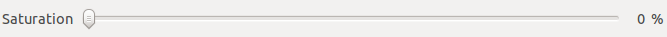
\includegraphics[width=\linewidth]{saturation_00}
	}
	
	\subfloat[Nivell de càrrega al 89\%]{\label{saturation_89}
		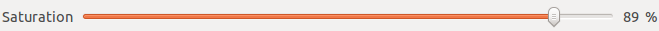
\includegraphics[width=\linewidth]{saturation_89}
	}
	
	\subfloat[Nivell de càrrega al 94\%]{\label{saturation_94}
		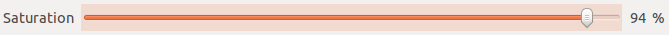
\includegraphics[width=\linewidth]{saturation_94}
	}

	\caption{Barra lliscant de càrrega en diferents posicions.}
    \label{fig:comparacio:barra}
\end{figure}

\FloatBarrier

%====================================================================================%
% Recepció de valors monitoritzats
%====================================================================================%
\subsubsection{Recepció de valors monitoritzats}\label{cap:imp:com:serie:rec:monitor}

Per poder realitzar la recepció de moltes dades pel port serie, es fa necessari deixar algun proces escoltant contínuament al port serie, però no podem permetre que el nostre programa es dediqui exclusivament a aquesta tasca, ja que tenim una interfície que hem d'atendre, gràfiques a dibuixar, i botons, que poden ser activats o desactivats. Per aquesta raó primer de tot creem un temporitzador, que permeti fer aquesta recepció de manera intermitent, deixant temps per atendre les altres tasques. Per fer això creem aquest temporitzador, i li assignem un disparador, que activarà la funció \emph{get\_periodical\_data} cada cop que passi el temps que li indiquem (codi \ref{cap:imp:com:serie:rec:monitor:trig:code}).

\begin{code_python}{Temporitzador i disparador per rebre dades del port serie}{cap:imp:com:serie:rec:monitor:trig:code}
timer_data = QtCore.QTimer()
    
# Periodical tasks
QtCore.QObject.connect(self.timer_data, QtCore.SIGNAL("timeout()"), self.get_periodical_data)
\end{code_python}

Peró aquesta declaració que hem creat no s'activa per si sola, sinó que hem d'engegar el temporitzador quan el necessitem, per tant cada cop que necessitem rebre informació de un llaç de control, o que volem una llista dels diferents llaços que hi ha al bus CAN al clicar el botó adequat (i després de realitzar codi que hem explicat en anteriors seccions) acabarà cridant a la funció \emph{get\_periodical\_data} (codi \ref{cap:imp:com:serie:rec:monitor:perio:code}).

Aquesta funció és l'encarregada de comprovar que la temporització funciona correctament, reactivant-la o parant-la en el moment oportú. El que fa primer de tot es comprovar que un dels botons que indiquen rebre informació estigui premut (aquests botons es queden premuts fins que no es torna a clicar per segon cop), en cas contrari ha d'aturar aquesta periodicitat i per tant ja no activa el temporitzador.
Un cop sap que realment es vol rebre informació, comprova que s'hagi dibuixat ja la informació que hi havia pendent, si ja s'ha dibuixat torna a rebre dades cridant a la funció \emph{recive\_data} (codi de la funció \ref{cap:imp:com:serie:rec:monitor:rx:code}). Això és així per crear una zona d'exclusió mútua (també anomenada Mutex), que evitarà que intentem dibuixar la gràfica de dades que estan a mig omplir.
I finalment reactiva el temporitzador per tornar a executar la mateixa funció.

\begin{code_python}{Codi per reactivar l'adquisició de dades}{cap:imp:com:serie:rec:monitor:perio:code}
def get_periodical_data(self):
    """Updates the data"""
    if not self.pushButton_monitor.isChecked() and not self.pushButton_reload.isChecked():
        return
    
    if self.updated_data == 0 :
        # recive new serial data
        self.recive_data()
        
    # activate the periodical reception of data
    self.timer_data.start(DATA_TIME)
\end{code_python}

Finalment la funció encarregada en rebre les dades pel port serie és la funció \emph{recive\_data} (codi \ref{cap:imp:com:serie:rec:monitor:rx:code}). Aquesta funció procura agafar tota la informació que hi hagi pendent al buffer d'entrada del port serie. Tenint en compte que el dispositiu \Monitor i el \SensorActuador envien aquesta informació cada 10 milisegons, i nosaltres fem lectures com a mínim cada 5 milisegons, tenim temps per fer la lectura i seguir executant altres codis. Primer de tot busca el byte de capçalera; aquest byte és un 0x01 que està al principi de tots els missatges que el dispositiu ens envia. Un cop ha trobat aquest byte sap que te les dades alineades, i pot prosseguir a llegir el numero de bytes que li correspongui (segons estigui en mode PC$->$\SensorActuador o PC$->$\Monitor llegirà 23 o 71 bytes respectivament). Ja amb el numero de bytes llegits, comprova si el botó de monitorització esta premut, per tal de agafar les dades per dibuixar la gràfica o passar a rebre la llista de dispositius (el codi que falta està en la secció \ref{cap:imp:com:serie:rec:devices}, codi \ref{cap:imp:com:serie:rec:devices:code}).

En la majoria de casos aquest botó si que està premut, i per tant agafa els bytes en l'ordre correcte per formar totes les variables necessàries, prepara el text per mostrar per pantalla i l'escriu en la part inferior del programa (figura \ref{fig:comparacio:valors}). Després afegeix als arrays el nou valor, i en treu un si ha arribat al màxim.
Després modifica els valors que apareixen en les estadístiques i habilita la zona d'exclusió.

\begin{code_python}{Codi per rebre els valors monitoritzats}{cap:imp:com:serie:rec:monitor:rx:code}
def recive_data(self):
    """Get messages from the serial port"""
    # read all available data
    while self.ser.inWaiting() > self.INPUT_DATA_SIZE+1:
        data = array.array('c')
        # search the header
        data.append(self.ser.read(1))
        while data[0] != chr(1):
            data[0] = self.ser.read(1)
            
        # wait for all available data
        while self.ser.inWaiting() < (self.INPUT_DATA_SIZE-1):
            time.sleep(0.03);
            
        # recives data
        data = self.ser.read(self.INPUT_DATA_SIZE-1)
        
        # prove if you want graphical data
        if self.pushButton_monitor.isChecked():
            # decodes the data
            t  = struct.unpack('I', data[3]+data[2]+data[1]+data[0])
            r  = struct.unpack('f', data[4]+data[5]+data[6]+data[7])
            x0 = struct.unpack('f', data[8]+data[9]+data[10]+data[11])
            x1 = struct.unpack('f', data[12]+data[13]+data[14]+data[15])
            u  = struct.unpack('f', data[16]+data[17]+data[18]+data[19])
            
            self.time = t[0]*25e-9
            
            # prepare the string output
            aux_str  = " t = "+str(self.time)+"\t"
            aux_str += " r = "+str(r[0])+"\t"
            aux_str += " u = "+str(u[0])+"\t"
            aux_str += " x1 = "+str(x1[0])+"\t"
            aux_str += " x0 = "+str(x0[0])+"\n"
            # print string output
            self.textBrowser.insertPlainText(aux_str)
            
            # append data to the arrays
            self.graf_t.append(self.time)
            self.graf_r.append(r[0])
            self.graf_x0.append(x0[0])
            self.graf_x1.append(x1[0])
            self.graf_u.append(u[0])
            
            # remove one value if the arrays have maximum length
            if self.graf_t.buffer_info()[1] >= NUM_SAMPLES:
                self.graf_t.pop(0)
                self.graf_r.pop(0)
                self.graf_x0.pop(0)
                self.graf_x1.pop(0)
                self.graf_u.pop(0)
                  
            # reload number of samples lavel
            self.label_samples_value.setText(str(self.graf_t.buffer_info()[1]))
            # reload number of waiting chars in serial rx buffer
            self.label_rx_buff_value.setText(str(self.ser.inWaiting()))

            # reload mutex area
            self.updated_data = 1
\end{code_python}

\begin{figure}[ht!]
	\subfloat[Rebent els valors d'una monitorització.]{\label{valors_rebent}
		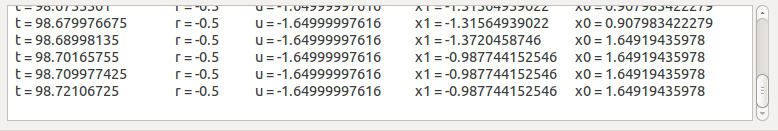
\includegraphics[width=\linewidth]{valors_rebent}
	}
	
	\subfloat[Havent finalitzat una monitorització.]{\label{valors_final}
		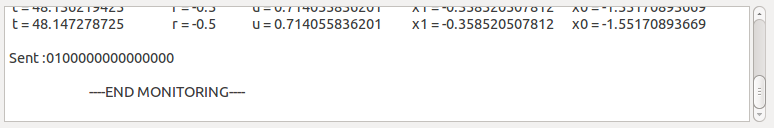
\includegraphics[width=\linewidth]{valors_final}
	}

	\caption{Espai de text per valors monitoritzats.}
    \label{fig:comparacio:valors}
\end{figure}

\FloatBarrier

%====================================================================================%
% Recepció de llista de dispositius
%====================================================================================%
\subsubsection{Recepció de llista de dispositius}\label{cap:imp:com:serie:rec:devices}

Per la recepció dels identificadors dels llaços de control com hem vist en l'apartat anterior \ref{cap:imp:com:serie:send:devices} s'activa la mateixa funció periòdica per rebre informació, per tant el codi que segueix és la continuació de la funció vista anteriorment \emph{recive\_data} (codi \ref{cap:imp:com:serie:rec:monitor:rx:code}).
Per tant seguint l'execució d'aquesta funció abans mencionada, comprovem si el byte 20 de les dades que ens arriben està a valor dos. En aquest cas significa que en el següent byte ve el nombre de identificadors diferents de mida un byte que el segueixen. Així que comprova un a un si ja es trobaven a la llista, i si no és així els afegeix.

\begin{code_python}{Codi per rebre la llista de dispositius }{cap:imp:com:serie:rec:devices:code}
....
# prove if there are available id's
if (self.actionPC_Monitor.isChecked() and data[20] == chr(2)):
    # if it is true, looks how much id's
    i  = struct.unpack('B', data[21])

    if i[0] < STACK_SIZE:
        for z in range(i[0]):
            new_device = struct.unpack('B', data[z+22])
            new_string = str(new_device[0])
            
            llista = self.listWidget_link.findItems(new_string, QtCore.Qt.MatchExactly)
            if len(llista) == 0:
                self.listWidget_link.addItem(new_string)
\end{code_python}

Es poden veure com a exemple algunes captures de pantalla de la llista abans de començar a demanar-li els identificadors (figura \ref{llista_cap}), actualitzant la llista en un bus amb dos llaços de control (figura \ref{llista_algun}), i la ultima imatge havent demanat la llista en un bus on existien varis llaços de control (figura \ref{llista_molts}).

\begin{figure}[ht!]
	\subfloat[Abans de demanar la llista.]{\label{llista_cap}
		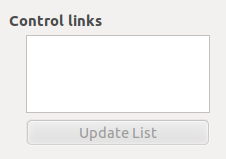
\includegraphics[width=0.3\linewidth]{llista_cap}
	}
	\subfloat[Amb dos llaços al bus CAN.]{\label{llista_algun}
		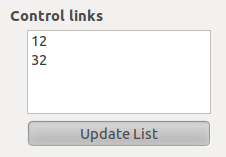
\includegraphics[width=0.3\linewidth]{llista_algun}
	}
	\subfloat[Amb molts llaços al bus CAN]{\label{llista_molts}
		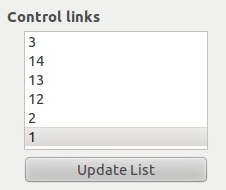
\includegraphics[width=0.3\linewidth]{llista_molts}
	}

	\caption{Llista de llaços de control al bus CAN.}
    \label{fig:comparacio:llista}
\end{figure}

\FloatBarrier

%====================================================================================%
% Generació de gràfiques en temps real
%====================================================================================%
\subsection{Generació de gràfiques en temps real}\label{cap:imp:gen:graph}

Generar aquestes gràfiques és un dels propòsits més importants del programa, i per tant ha de ser prou ràpida per no saturar el programa però al mateix temps donar una sensació visual de moviment.
Aquesta generació està associada a un temporitzador especific, enllaçat a un disparador que activa la funció \emph{update\_graph} (codi \ref{cap:imp:gen:graph:code}).
Aquest temporitzador s'activa només quan es prem el botó de monitorització, vist en la secció \ref{cap:imp:com:serie:send:monit}.

\begin{code_python}{Temporitzador i disparador per dibuixar la gràfica}{cap:imp:gen:graph:trig:code}
timer_graph = QtCore.QTimer()

# Periodical tasks
QtCore.QObject.connect(self.timer_graph, QtCore.SIGNAL("timeout()"), self.update_graph)
\end{code_python}

Un cop s'ha activat el temporitzador que crida aquesta funció, primer de tot comprova que hi hagi dades noves per dibuixar i que no s'estiguin modificant en aquest precís instant (això s'ha vist en la secció de recepció de dades \ref{cap:imp:com:serie:rec:monitor}). Si les dades que hi ha han estat actualitzades dibuixa primer les línies verticals i horitzontals que hi ha darrera dels plots. I després comprova un a un si hi ha marcada la opció de dibuixar els diferents plots (referència, primera i/o segona integral i valor d'entrada; figura \ref{fig:comparacio:plots}); segons quins estiguin activats, els crea i dibuixa o no. Finalment prova de pintar tot el que ha generat, actualitza la variable \emph{frames per second} per indicar que s'ha fet un nou dibuix i es marca la variable per la zona d'exclusió mútua perquè es puguin seguir afegint dades als arrays.
Finalment comprova que encara es vulgui seguir dibuixant la gràfica i es reactiva la temporització.
        
\begin{code_python}{Codi per actualitzar la gràfica }{cap:imp:gen:graph:code}
def update_graph(self):
    """Updates the graph"""
    # looks for new data
    if self.updated_data == 1:
                  
        self.mplWidget.canvas.ax.set_xbound(self.time-XLIM, self.time)
        self.mplWidget.canvas.draw()

        try:
            #Draw the lines
            if self.checkBox_R.isChecked():
                self.referenceLine.set_data(self.graf_t, self.graf_r)
                self.mplWidget.canvas.ax.draw_artist(self.referenceLine)
            if self.checkBox_x0.isChecked():
                self.x0Line.set_data(self.graf_t, self.graf_x0)
                self.mplWidget.canvas.ax.draw_artist(self.x0Line)
            if self.checkBox_U.isChecked():
                self.uLine.set_data(self.graf_t, self.graf_u)
                self.mplWidget.canvas.ax.draw_artist(self.uLine)
            if self.checkBox_x1.isChecked():
                self.x1Line.set_data(self.graf_t, self.graf_x1)
                self.mplWidget.canvas.ax.draw_artist(self.x1Line)
        except AssertionError:
            pass
            
        try:
            self.mplWidget.canvas.blit(self.mplWidget.canvas.ax.bbox)
        except AttributeError:
            pass
        
        self.fps = self.fps+1
        
        self.updated_data = 0
        
    if self.pushButton_monitor.isChecked() == 1:
        # activate the periodical update graph
        self.timer_graph.start(GRAPH_REFRESH)
\end{code_python}


\begin{figure}[ht!]
\begin{center}
	\subfloat[Abans alguns plots seleccionats.]{\label{alguns_seleccionats}
		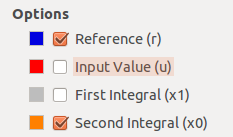
\includegraphics[width=0.35\linewidth]{alguns_seleccionats}
	}
	\subfloat[Amb tots els plots seleccionats.]{\label{tots_seleccionats}
		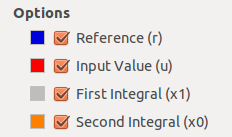
\includegraphics[width=0.35\linewidth]{tots_seleccionats}
	}
\end{center}
	\caption{Opció de plots per la gràfica.}
    \label{fig:comparacio:plots}
\end{figure}

\FloatBarrier

%====================================================================================%
% Exportar gràfica
%====================================================================================%
\subsection{Exportar gràfica}\label{cap:imp:exp:graph}

Exportar les gràfiques que s'estiguin monitoritzant en temps real és molt important, ja que gracies a això es pot guardar una captura de cada grup del laboratori, o generar imatges vectorials fàcilment introduïbles en articles o llibres (formats com .eps, .svg, .ps o .pdf).
Per poder generar aquestes imatges s'espera que es premi un botó, que està enllaçat mitjançant un disparador (codi \ref{cap:imp:exp:graph:trig:code}) a la funció que genera la imatge \emph{save\_image} (codi \ref{lab:imp:exp:graph:code}).

\begin{code_python}{Disparador per exportar la gràfica}{cap:imp:exp:graph:trig:code}
QtCore.QObject.connect(self.pushButton_save, QtCore.SIGNAL(_fromUtf8("clicked()")), self.save_image)
\end{code_python}

Un cop han activat aquesta funció primerament s'obra una finestra nova on es pot introduir el nom del nou fitxer a crear (figura \ref{exportant_nom}). A part de poder introduir el nom, podem llistar tots els fitxers dels diferents tipus que el programa és capaç de exportar, que hi hagin en el directori que estem observant. Per aquest motiu en la creació de la finestra apareixen descripcions d'aquests tipus de fitxers (figura \ref{exportant_tipus}).

\figuremacroW{exportant_nom}{Finestra per posar nom a la gràfica exportada}{}{0.9}

\figuremacroW{exportant_tipus}{Tipus de fitxer als que es pot exportar}{}{0.5}

Un cop l'usuari ha introduït el nom i clicat a acceptar començarem a generar una gràfica nova des de zero. Comprovarem un a un tots els plots que hem de dibuixar, afegint a la gràfica els que calguin.
Tot seguit indicarem quin rang de valors volem dibuixar, i posarem títol, subtítol, i noms als diferents eixos (tots aquests textos són traduïts a l'idioma que hi hagi seleccionat en el programa).
Després assigna algunes de les mides del dibuix, i finalment intenta guardar la imatge amb el nom i format que li hagim indicat anteriorment. Si per alguna raó fallés en aquesta tasca, procuraria guardar-lo en format \emph{.svg}.
Al acabar de generar la imatge aquesta gràfica nova es neteja per alliberar la memòria.

Un cop finalitzat el programa, el resultat de la captura de imatges és el que es pot observar en la figura \ref{fig:comparacio:graph}, en la que apareix una gràfica generada en anglès, amb totes les línies, i una altre en català només amb les línies de referència i de sortida del doble integrador.

\begin{figure}[ht!]
	\subfloat[Amb textos en anglès, totes els plots i en format PDF.]{\label{necs_di_graph}
		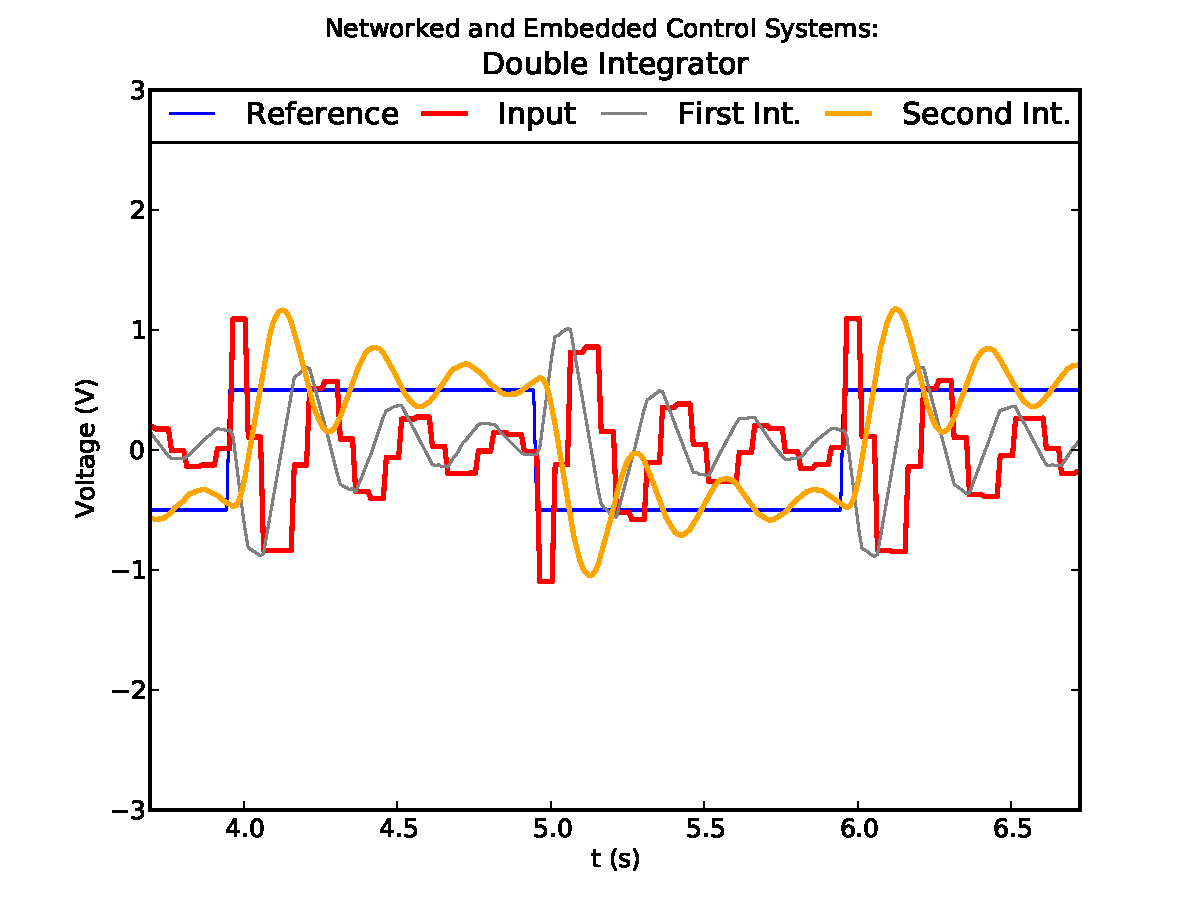
\includegraphics[width=0.88\linewidth]{necs_di_graph}
	}
	\\
	\subfloat[Amb el bus CAN carregat de missatges, amb textos en català, només amb plots de referència i segona integral i en format PDF.]{\label{di_saturat_ref_segona_cat}
		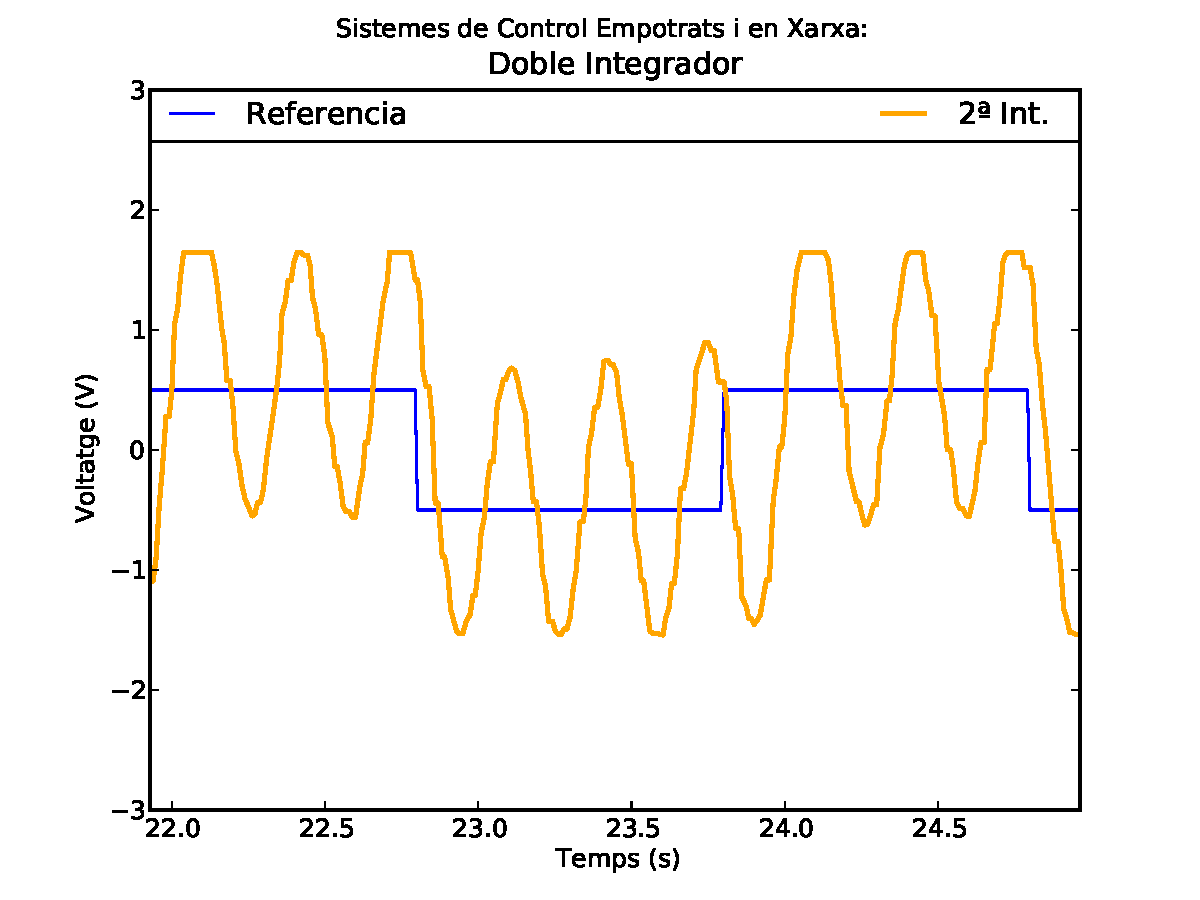
\includegraphics[width=0.88\linewidth]{di_saturat_ref_segona_cat}
	}

	\caption[Diferents gràfiques generades amb el programa \DCSMonitor]{Diferents gràfiques generades amb el programa \DCSMonitor del control d'un doble integrador.}
    \label{fig:comparacio:graph}
\end{figure}

\begin{code_python}{Codi per generar imatge d'una gràfica}{lab:imp:exp:graph:code}
def save_image(self):
    """Exports the graph into an image"""
    # open the dialog and get the selected file
    file_one = QtGui.QFileDialog.getSaveFileName(
         self,
         QtGui.QApplication.translate(
            "MainWindow", 
            "Supported formats:", 
            None, 
            QtGui.QApplication.UnicodeUTF8)+
            " emf, eps, pdf, png, ps, raw, rgba, svg, svgz", 
         "",
         "Enhanced MetaFile \t.emf (*.emf);; "+
         "Encapsulated PostScript \t.eps (*.eps);; "+
         "Portable Document Format \t.pdf (*.pdf);; "+
         "Portable Network Graphics \t.png (*.png);;"+
         "PostScript \t.ps (*.ps);; "+
         "RAW image file \t.raw (*.raw);; "+
         "Red Green Blue Alpha \t.rgba (*.rgba);; "+
         "Scalable Vector Graphics \t.svg (*.svg);; "+
         "Scalable Vector Graphics compressed \t.svgz (*.svgz)")
    # if a file is selected
    if file_one:
        # update the lineEdit text with the selected filename
        self.textBrowser.append(
            QtGui.QApplication.translate(
                "MainWindow", 
                "Saving to ", 
                None, 
                QtGui.QApplication.UnicodeUTF8
                )+file_one)

        plt.clf()
        # adding different plots if required
        if self.checkBox_R.isChecked():
            lines = plt.plot(self.graf_t, self.graf_r)
            plt.setp(lines[0], 
                     lw=1, 
                     label=str(
                        QtGui.QApplication.translate(
                            "MainWindow", 
                            "Reference",  
                            None, 
                            QtGui.QApplication.UnicodeUTF8)), 
                    color = 'blue')
            
        if self.checkBox_U.isChecked():
            lines = plt.plot(self.graf_t, self.graf_u)
            plt.setp(lines[0], 
                     lw=2, 
                     label=str(
                        QtGui.QApplication.translate(
                            "MainWindow", 
                            "Input",      
                            None, 
                            QtGui.QApplication.UnicodeUTF8)), 
                     color='red')
            
        if self.checkBox_x1.isChecked():
            lines = plt.plot(self.graf_t, self.graf_x1)
            plt.setp(lines[0], 
                     lw=1, 
                     label=str(
                        QtGui.QApplication.translate(
                            "MainWindow", 
                            "First Int.",  
                            None, 
                            QtGui.QApplication.UnicodeUTF8)), 
                     color='grey')
            
        if self.checkBox_x0.isChecked():
            lines = plt.plot(self.graf_t, self.graf_x0)
            plt.setp(lines[0], 
                     lw=2, 
                     label=str(
                        QtGui.QApplication.translate(
                            "MainWindow", 
                            "Second Int.", 
                            None, 
                            QtGui.QApplication.UnicodeUTF8)), 
                     color='orange')

        plt.axis([self.graf_t[0], self.graf_t[-1], -3, 3])
        
        plt.title(str(
            QtGui.QApplication.translate(
                "MainWindow", 
                "Double Integrator", 
                None, 
                QtGui.QApplication.UnicodeUTF8)))
        
        plt.suptitle(str(
            QtGui.QApplication.translate(
                "MainWindow", 
                "Networked and Embedded Control Systems:", 
                None, 
                QtGui.QApplication.UnicodeUTF8)))
        
        plt.xlabel(str(
            QtGui.QApplication.translate(
                "MainWindow", 
                "t (s)", 
                None, 
                QtGui.QApplication.UnicodeUTF8)))
        
        plt.ylabel(str(
            QtGui.QApplication.translate(
                "MainWindow", 
                "Voltage (V)", 
                None, 
                QtGui.QApplication.UnicodeUTF8)))
        
        plt.legend(bbox_to_anchor=(0, 1, 1, 0), loc=1, ncol=6, mode="expand", borderaxespad=0.)
               
        filename = str(file_one)# + '.svg'
        try:
            plt.savefig(filename, dpi=300)
        except ValueError as e:
            print(e)
            self.textBrowser.append(str(e))
            self.textBrowser.append(
                QtGui.QApplication.translate(
                    "MainWindow", 
                    "Trying to save as .svg", 
                    None, 
                    QtGui.QApplication.UnicodeUTF8))
            
            filename = str(file_one) + '.svg'
            plt.savefig(filename, dpi=300)
            pass
        except ImportError as e:
            print(e)
            self.textBrowser.append(str(e))
            self.textBrowser.append(
                QtGui.QApplication.translate(
                    "MainWindow", 
                    "Trying to save as .svg", 
                    None, 
                    QtGui.QApplication.UnicodeUTF8))
            
            filename = str(file_one) + '.svg'
            plt.savefig(filename, dpi=300)
            pass
        except:
            self.textBrowser.append("Error al guardar la imatge")
        
        plt.clf()
\end{code_python}

\FloatBarrier

%====================================================================================%
% Mostrant estadístiques
%====================================================================================%
\subsection{Mostrant estadístiques}\label{cap:imp:estat}

Com en la part de disseny es va explicar, periòdicament anirem creant estadístiques per saber que tot funciona correctament. 
Els valors que ens interessa saber en cada instant són: 

\begin{itemize}
	\item Nombre de llaços de control que hi ha connectats al bus CAN.
	\item Imatges per segon que es mostren en la gràfica en temps real.
	\item Nombre de mostres per plot dibuixat.
	\item Nombre de bytes esperant al buffer d'entrada del port serie.
	\item Marca canviant per saber que les estadístiques s'estan actualitzant periòdicament.
\end{itemize}

Per fer que aquestes estadístiques s'actualitzin periòdicament, com hem vist en altres seccions primer de tot hem de crear un temporitzador, i tot seguit li assignarem un disparador que activará la funció \emph{update\_statistics} (codi del disparador, i activació de les estadístiques \ref{cap:imp:est:trig:code}).

\begin{code_python}{Temporitzador i disparador per actualitzar les estadístiques.}{cap:imp:est:trig:code}
timer_statistics = QtCore.QTimer()

# Periodical tasks
QtCore.QObject.connect(self.timer_statistics, QtCore.SIGNAL("timeout()"), self.update_statistics)

self.timer_statistics.start(STAT_REFRESH)
\end{code_python}

El que fa la funció \emph{update\_statistics} (codi \ref{lab:imp:estat:update:code}) és primer de tot comprovar que el port serie estigui degudament connectat, si no és així no modifica cap valor estadístic, en cas contrari comença a actualitzant el nombre de mostres de tots els plots, el nombre de bytes pendents al port serie, el nombre d'imatges per segon que estan apareixent a la gràfica (si aquesta està aturada, força un dibuix cada cop, per si hi ha algun problema), actualitza el valor canviant per indicar que aquesta funció està funcionant correctament, actualitza el nombre de llaços de control que hi ha al bus CAN i finalment torna a reactivar la funció al cap de mig segon.

\begin{code_python}{Codi per generar i actualitzar les estadístiques.}{lab:imp:estat:update:code}
def update_statistics(self):
    """Update value of labels in statistics"""
    if self.ser != 0:
        # reload number of samples lavel
        self.label_samples_value.setText(str(self.graf_t.buffer_info()[1]))
        # reload number of waiting chars in serial rx buffer
        self.label_rx_buff_value.setText(str(self.ser.inWaiting()))
        
        self.label_fps_value.setText(str(self.fps*2))
        
        self.fps = 0
        
        if self.pushButton_monitor.isChecked() == 0:
            self.force_update_graph()
            
        if self.label_Est_value.text() != '(>_<)':
            self.label_Est_value.setText('(>_<)')
        else:
            self.label_Est_value.setText('(o_o)')
        
        self.label_T_value.setText(str(self.listWidget_link.count()))
        
        self.timer_statistics.start(STAT_REFRESH)
\end{code_python}

Tot seguit es poden veure diferents captures del canvi que es produeix en les estadístiques, primer es veu quan encara no està connectat al port serie, després al connectar però no tractar les dades que ens envia el dispositiu, després un cop estem tractant les dades rebudes i dibuixant la gráfica en temps real, i per ultim un cop hem aturat la monitorització del llaç de control (figura \ref{fig:comparacio_estadistiques}).

\begin{figure}[ht!]
	\subfloat[Pendent de començar.]{\label{estadistiques_pendents}
		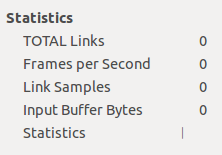
\includegraphics[width=0.24\linewidth]{estadistiques_pendents}
	}
	\subfloat[Connectat al dispositiu.]{\label{estadistiques_connect}
		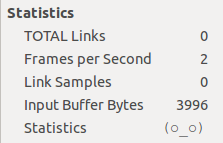
\includegraphics[width=0.24\linewidth]{estadistiques_connect}
	}
	\subfloat[Monitoritzant.]{\label{estadistiques_monitoritzant}
		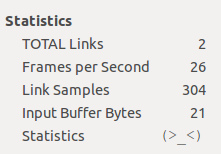
\includegraphics[width=0.24\linewidth]{estadistiques_monitoritzant}
	}
	\subfloat[Monitorització aturada.]{\label{estadistiques_desconnect}
		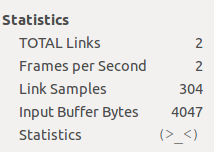
\includegraphics[width=0.24\linewidth]{estadistiques_desconnect}
	}
	\caption{Comparació dels valors estadístics.}
    \label{fig:comparacio_estadistiques}
\end{figure}

\FloatBarrier

%====================================================================================%
% Idiomes
%====================================================================================%
\subsection{Idiomes}\label{cap:imp:idi}

Un dels requisits que es buscava complir en el nou laboratori era que el programa visual fos multilingüe per tal de poder ser distribuït més fàcilment podent realitzar el laboratori en diferents països.

Així que el programa \DCSMonitor (que s'executa a l'ordinador) és capaç de mostrar tota la informació en varis idiomes, i és fàcilment ampliable ja que s'ha realitzat de forma estructurada per tal que seguint algunes instruccions es puguin generar més idiomes.

Com vam dir a l'apartat de disseny \ref{cap:dis:idi}, això ho hem aconseguit utilitzant una combinació de diferents eines amb les quals una rere l'altre ens generen el resultat desitjat. Tot seguit s'expliquen les diferents eines utilitzades, i com s'implementa cadascuna.

%====================================================================================%
% PyQT4
%====================================================================================%
\subsubsection{PyQT4}\label{cap:imp:idi:pyqt4}

Aquesta llibreria és l'encarregada de deixar-ho tot preparat perquè els textos del programa siguin traduits. Així que primerament, dintre de tot el codi del programa, es pot observar que tots els textos traduibles están envoltats amb la mateixa funció \emph{QtGui.QApplication.translate} (veure exemple en el codi \ref{lab:imp:idi:pyqt4:trans:example}).
Aquesta funció prepara tot l'entorn necessari per agafar tots aquests textos, i posteriorment mitjançant uns fitxers de traducció traduir en temps d'execució.
En aquest exemple li indiquem que la paraula "Sent : " volem que pugui ser traduïda, per tant cada cop que cridem aquesta funció amb aquesta estructura ens retornarà la paraula en l'idioma que tinguem carregat.

\begin{code_python}{Exemple de text per traduir}{lab:imp:idi:pyqt4:trans:example}
QtGui.QApplication.translate(
    "MainWindow", 
    "Sent : ", 
    None, 
    QtGui.QApplication.UnicodeUTF8)
\end{code_python}

Un cop tenim tot el codi amb els textos a traduir envoltats de la funció anterior, generarem les traduccions en fitxers \emph{.qm} amb els dos programes que explicarem més endavant (\Pylupdate \ref{cap:imp:idi:pylupdate4} i \Qtlinguist \ref{cap:imp:idi:qtlinguist}), i un cop generats només caldrà carregar executar el codi \ref{lab:imp:idi:pyqt:reload}.
Per tant cada cop que des de les preferències es seleccioni un idioma només carregarem el fitxer \emph{.qm} que desitgem.

\begin{code_python}{Canviant idioma}{lab:imp:idi:pyqt:reload}
QtGui.qApp.removeTranslator(self.translator)
self.translator.load('dcsmmainwindow_es.qm')
QtGui.qApp.installTranslator(self.translator)
self.retranslateUi(self)
\end{code_python}

%====================================================================================%
% Pylupdate4
%====================================================================================%
\subsubsection{Pylupdate4}\label{cap:imp:idi:pylupdate4}

Un cop tenim tot el codi del programa \DCSMonitor preparat amb els textos a traduir de la forma que s'ha comentat en la secció \ref{cap:imp:idi:pyqt4}, és hora d'utilitzar aquesta eina.
Aquest programa recorre els diferents codis que li indiquem, buscant aquells textos preparats per traduir. Un cop trobats genera un fitxer de traduccions seguint el format \emph{.ts}.
Aquesta acció s'ha de executar per cada idioma a traduir que vulguem per tant es posa el codi per generar els quatre fitxers de traducció que actualment tenim (codi \ref{cap:imp:idi:lupdate}).
Els fitxers generats poden ser editats amb varis programes, i posteriorment es generarà un nou fitxer amb extensió \emph{.qm}.

\begin{code_bash}{Crear fitxers per traduccions}{cap:imp:idi:lupdate}
pylupdate4 dcsmmainwindow.py main_dcsm.py -ts dcsmonitor_en.ts
pylupdate4 dcsmmainwindow.py main_dcsm.py -ts dcsmonitor_es.ts
pylupdate4 dcsmmainwindow.py main_dcsm.py -ts dcsmonitor_ca.ts
pylupdate4 dcsmmainwindow.py main_dcsm.py -ts dcsmonitor_fr.ts
\end{code_bash}


%====================================================================================%
% QtLingüist
%====================================================================================%
\subsubsection{QtLingüist}\label{cap:imp:idi:qtlinguist}

Gracies a aquest programa podem editar un a un els diferents fitxers generats anteriorment (secció \ref{cap:imp:idi:pylupdate4}), i un cop hem traduit totes les paraules li podem demanar que ens generi el fitxer de traduccions, que és capaç de carregar la llibreria \PyQT com hem dit en la secció \ref{cap:imp:idi:pyqt4}.
En la figura següent (figura \ref{qtlinguist}) es pot veure l'entorn d'edició d'un fitxer, en la part central les paraules marcades en verd ja traduides i la paraula seleccionada que apareix per traduir una mica més abaix.

\figuremacro{qtlinguist}{Utilitzant \Qtlinguist}{Programa que ens permet editar un fitxer de traduccions \emph{.ts}, i generar el fitxer \emph{.qm}}



%====================================================================================%
% Resultat
%====================================================================================%
\subsubsection{Resultat}\label{cap:imp:idi:res}

Un cop realitzats tots els passos indicats en aqueta secció, tindrem els quatre fitxers de traducció següents:
\begin{itemize}
	\item dcsmonitor\_en.qm
	\item dcsmonitor\_es.qm
	\item dcsmonitor\_ca.qm
	\item dcsmonitor\_fr.qm
\end{itemize}

I ja podrem canviar l'idioma anant a les preferències del programa (Figura \ref{Preferencies}) i seleccionant un dels idiomes llistats.

\figuremacroW{Preferencies}{Preferències del programa DCSMonitor}{Des de les preferències podem seleccionar l'idioma}{0.3}

Tot seguit es poden observar alguns dels canvis que s'efectuen al canviar l'idioma (Figura \ref{fig:comparacio_idiomes})

\begin{figure}[ht!]
	\subfloat[Labels en Català]{\label{idioma_ca}
		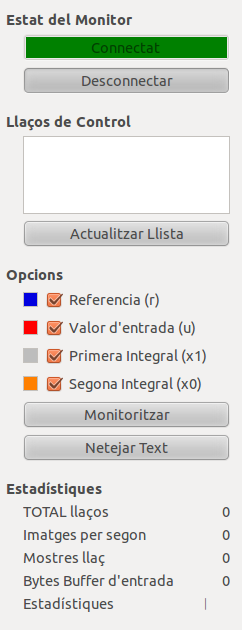
\includegraphics[scale=0.4]{idioma_ca}
		%\figuremacroW{labels_ca}{Labels en Català}{}{0.4}
	}
	\subfloat[Labels en Espanyol]{\label{idioma_es}
		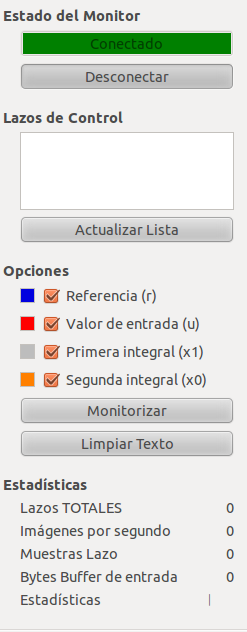
\includegraphics[scale=0.4]{idioma_es}
		%\figuremacroW{labels_es}{Labels en Espanyol}{}{0.4}
	}
	\subfloat[Labels en Anglés]{\label{idioma_en}
		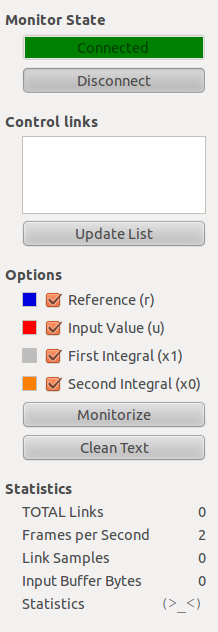
\includegraphics[scale=0.4]{idioma_en}
		%\figuremacroW{labels_en}{Labels en Anglés}{}{0.4}
	}
	\subfloat[Labels en Francés]{\label{idioma_fr}
		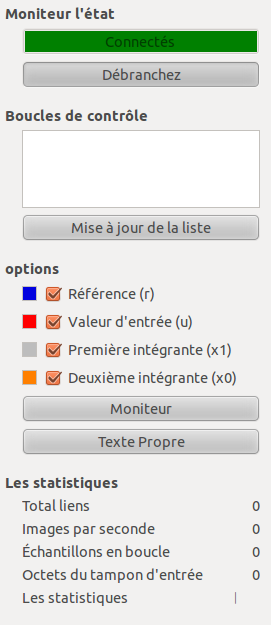
\includegraphics[scale=0.4]{idioma_fr}
		%\figuremacroW{labels_fr}{Labels en Francés}{}{0.4}
	}
	\caption{Comparació dels labels entre diferents idiomes.}
    \label{fig:comparacio_idiomes}
\end{figure}

\FloatBarrier

%====================================================================================%
% dsPIC
%====================================================================================%
\section{dsPIC}\label{lab:imp:dspic:monitor}

Aquesta secció pretén explicar les parts del codi més importants dels microcontroladors dsPIC. Tot el sistema està basat en el RTOS Erika Enterprise, així que la majoria de les funcions són tasques que són activades, o es realitzen periòdicament mitjançant alarmes.

Aquesta manera de programar permet la concurrència entre diferents tasques, el que comporta una major atenció als diferents tipus de accions que el microcontrolador ha de dur a terme.

En els microcontroladors que utilitzem aquesta concurrència es en el mateix nucli, per tant tot s'executa en serie, però aquest sistema operatiu garanteix l'execució de totes les tasques.

Tot seguit es poden veure les diferents parts més importants d'aquests programes.

%====================================================================================%
% Tasques TODO
%====================================================================================%
\subsection{Tasques en Erika}\label{lab:imp:dspic:monitor:tasks}

El RTOS Erika ens ofereix una serie d'eines per generar d'alguna manera tasques que s'executin periòdicament. En el nostre laboratori ens aprofitem d'aquesta facilitat i moltes de les funcions que fem servir en els diferents dispositius estan realitzades d'aquesta manera.

Per tal d'aconseguir això primerament s'han de declarar les tasques que el nostre Sistema Operatiu podrà executar. Per això existeix un fitxer anomenat \emph{conf.oil} en el qual hem d'avisar a RT-Druid de la creació de les tasques que necessitem, a les quals se'ls pot assignar una prioritat diferent i temps màxim d'atenció entre d'altres opcions. També es necessari indicar-li quin dispositiu volem programar, amb quin programador, quins codis formaran part del SO, i altres qüestions que podem configurar. 

Tot seguit es posa a mode d'exemple el fitxer \emph{conf.oil} necessari per programar un dispositiu que només té la tasca de supervisió (aquesta tasca enviava informació d'estat a l'ordinador via RS232).

En el codi \ref{lab:imp:dspic:monitor:tasks:oil}, es pot veure la declaració del nostre sistema indicant-li el microcontrolador que usarem, els fitxers que formaran part del codi, i finalment la declaració de la tasca \emph{TaskSupervision} amb una prioritat de valor dos (valor més alt indica major prioritat), li donem també el máxim de temps per ser executada i que volem que la administri completament el Sistema Operatiu.

Més abaix creem una alarma per poder executar aquesta tasca de manera periòdica en cas de necessitar-ho.


\begin{code_c}{Exemple de declaració d'una tasca en el fitxer conf.oil}{lab:imp:dspic:monitor:tasks:oil}
CPU mySystem {

	OS myOs {
		EE_OPT = "DEBUG";

		CPU_DATA = PIC30 {
			APP_SRC = "setup.c";
			APP_SRC = "uart_dma.c";
			APP_SRC = "e_can1.c";
			APP_SRC = "code.c";
			MULTI_STACK = FALSE;
			ICD2 = TRUE;
		};

		MCU_DATA = PIC30 {
			MODEL = PIC33FJ256MC710;
		};

		BOARD_DATA = EE_FLEX {
			USELEDS = TRUE;
		};

		
		KERNEL_TYPE = EDF { NESTED_IRQ = TRUE; TICK_TIME = "25ns";};
		
	};

	TASK TaskSupervision {
		REL_DEADLINE = "0.1s";
		PRIORITY = 2;
		STACK = SHARED;
		SCHEDULE = FULL;
	};

	COUNTER myCounter;
	
	ALARM AlarmSupervision {
		COUNTER = "myCounter";
		ACTION = ACTIVATETASK { TASK = "TaskSupervision"; };
	};
}; 
\end{code_c}

Un cop tenim ben definit l'entorn del nostre Sistema Operatiu ja només cal utilitzar les tasques dintre del programa (codis d'exemple \ref{lab:imp:dspic:monitor:tasks:interact}). Per poder posar en marxa una tasca RT-Druid ens dona la funció \emph{ActivateTask(nom de la tasca)}, amb la qual només s'executarà un cop. 

En el cas de voler activat aquesta tasca periódicament podem activar una alarma amb la funció \emph{SetRelAlarm(AlarmType AlarmID, TickType increment, TickType cycle)} en la qual li indiquem el nom de l'alarma a executar, el temps d'espera per executar-la i el temps entre cicles d'execució. Finalment si en algun moment volguessin aturar aquesta alarma cíclica només hauríem de cridar la funció \emph{CancelAlarm(AlarmType AlarmID)}.

\begin{code_c}{Codis per interactuar amb tasques}{lab:imp:dspic:monitor:tasks:interact}
// Active one execution of a task
ActivateTask(TaskSupervision);

//Data is sent to the PC every 10ms
SetRelAlarm(AlarmSupervision, 1000, 10);

// Stops the periodiciti of a task
CancelAlarm(AlarmSupervision);
\end{code_c}


%====================================================================================%
% Comunicació sèrie
%====================================================================================%
\subsection{Comunicació serie RS232}\label{lab:imp:dspic:monitor:serie}

En aquest apartat explicarem com s'ha implementat la comunicació serie per RS232 que es va dissenyar en la secció \ref{cap:dis:comSer}. Recordem que els dos dispositius capaços d'interaccionar mitjançant aquesta tecnologia són el \Monitor i el \SensorActuador, per tant s'explicaran els codis d'aquests relacionats amb la comunicació serie.

%====================================================================================%
% Recepció de senyals de control
%====================================================================================%
\subsubsection{Recepció de senyals de control}\label{lab:imp:dspic:monitor:ser:rec}

Com hem explicat en la secció anterior \ref{cap:dis:comSer}, el dispositiu \Monitor ha de ser capaç de rebre diferents instruccions del programa \DCSMonitor per tal de poder posar en marxa certes accions.

Aquestes instruccions estan numerades i les dues parts de la comunicació han de coneixer-la, per tant primer de tot en el codi del \Monitor cal declarar aquests valors:

\begin{code_c}{Declaració dels valors dels senyals de control}{lab:imp:dspic:monitor:ser:define:signals}
#define SIGNAL_STOP			1
#define SIGNAL_MONITOR		0
#define SIGNAL_PERCENT		2
#define SIGNAL_DEVICES		4
\end{code_c}

Per tal de rebre els missatges per el port sèrie RS232 es va observar el mode de funcionament de la recepció dels missatges CAN i es va utilitzar la mateixa metodologia, creant una funció que s'executés cada cop que el port sèrie s'omplís amb 8 bytes. Aquesta funció seria la encarregada de comprovar el primer dels 8 bytes del missatge, i realitza una o altre acció depenent de la taula que s'ha mostrat anteriorment \ref{tab:ids:rs232}.

Tot seguit es pot veure la funció que rep la interrupció del buffer d'entrada del port sèrie:

\begin{code_c}{Interrupció buffer del port sèrie}{lab:imp:dspic:monitor:ser:int:in:code}
// Input serial buffer interrupt
ISR2(_DMA5Interrupt) //NOTE: Disabled when IEC3bits.DMA5IE = 0;
{
	float *p_k0=(float *)&InBufferA[0];
	unsigned long id_link;

	/*Code to update received data*/
	k_updated[0]= *(p_k0);
	k_updated[1]= *(p_k0+1);

	switch (InBufferA[0])
	{
	case SIGNAL_MONITOR:

		id_link = (unsigned long) InBufferA[7]<<2;
		// Generating id's for a control plant
		ID_TO_ACTUATOR 		= CONTROL_MESSAGE 			| GENERAL_PRIORITY | id_link;
		ID_FROM_SENSOR		= GRANTED_SENSOR_MESSAGE 	| GENERAL_PRIORITY | id_link;
		ID_REFERENCE		= GENERAL_PURPOSE_MESSAGE 	| GENERAL_PRIORITY | id_link | REFERENCE_MESSAGE;
		ID_SUPERVISOR		= GENERAL_PURPOSE_MESSAGE 	| GENERAL_PRIORITY | id_link | SUPERVISOR_MESSAGE;

		// Activating filters for different message id's
		//ecan1WriteRxAcptFilter(filter, id, exide, buffer, masc)
		ecan1WriteRxAcptFilter(0x0,ID_FROM_SENSOR	,0x1,0x1,0x2);
		ecan1WriteRxAcptFilter(0x1,ID_TO_ACTUATOR	,0x1,0x2,0x2);
		ecan1WriteRxAcptFilter(0x2,ID_REFERENCE		,0x1,0x3,0x2);
		ecan1WriteRxAcptFilter(0x3,ID_SUPERVISOR	,0x1,0x4,0x2);
		CancelAlarm(AlarmSupervision);
		// Starts sending supervision messages
		SetRelAlarm(AlarmSupervision, 1000, 10);
		monitoring = 1;
		break;

	case SIGNAL_PERCENT:
		// Starts to generate useless CAN messages
		CancelAlarm(AlarmCANUseless);
		SetRelAlarm(AlarmCANUseless, 1000,101-(InBufferA[7]));
		break;

	case SIGNAL_MONITOR+SIGNAL_STOP:
		// Stops the reception of control messages
		ecan1DisableRXFilter(0x0);
		ecan1DisableRXFilter(0x1);
		ecan1DisableRXFilter(0x2);
		ecan1DisableRXFilter(0x3);
		// If is not listing devices, stops to send supervisions
		if (!listing) CancelAlarm(AlarmSupervision);
		LATBbits.LATB14 = 0;
		monitoring = 0;
		break;

	case SIGNAL_PERCENT+SIGNAL_STOP:
		// Stops the generation of usless messages
		CancelAlarm(AlarmCANUseless);
		break;

	case SIGNAL_DEVICES:
		// Activate filter 4 to put all CAN messages into buffer 5
		ecan1WriteRxAcptFilter(0x4,0x00000000,0x1,0x5,0x1);
		SetRelAlarm(AlarmSupervision, 1000, 10);
		listing = 1;
		break;

	case SIGNAL_DEVICES+SIGNAL_STOP:
		// Desactivate filter 4
		ecan1DisableRXFilter(0x4);
		// If is not monitoring devices, stops to send supervisions
		if (!monitoring) CancelAlarm(AlarmSupervision);
		LATBbits.LATB14 = 0;
		listing = 0;
		break;

	default:
		break;
	}

	IFS3bits.DMA5IF = 0; // Clear the DMA1 Interrupt Flag
}
\end{code_c}

%====================================================================================%
% Recepció de senyals de control
%====================================================================================%
\subsubsection{Enviament de dades}\label{lab:imp:dspic:monitor:ser:send}

Tant el dispositiu \Monitor com el dispositiu \SensorActuador compten amb la informació periòdica d'algun llaç de control. Aquesta informació es va emmagatzemant temporalment per enviar-les cada 10 ms al programa \DCSMonitor.

Per realitzara aquesta tasca periòdicament el \SensorActuador activa una alarma al iniciar l'execució, el \Monitor en canvi, espera a que el programa \DCSMonitor li indiqui (codi \ref{lab:imp:dspic:monitor:ser:send:alarm})

\begin{code_c}{Alarma de supervisió}{lab:imp:dspic:monitor:ser:send:alarm}
//Data is sent to the PC every 10ms
SetRelAlarm(AlarmSupervision, 1000, 10);
\end{code_c}

La informació que envien els diferents dispositius varía, així el \SensorActuador envia només 23 bytes, amb els valors del temps, referència, entrada i primera i segona integral. En canvi el \Monitor envia 71 bytes, els quals porten la mateixa informació que hem dit, però poden incloure'n més. En aquest cas afegeixen els diferents identificadors de llaç de control, existents al bus CAN.

En el codi següent es pot veure la part comuna a tots dos codis, i una part que és única del dispositiu \Monitor, en la que comprova si hi ha identificadors a la pila, per cada identificador que veu incrementa el valor del byte 22, i guarda en les següents posicions els identificadors que va trobant. Al final posa el byte 21 a 2, per indicar-li al programa \Monitor que li està enviant identificadors (codi \ref{lab:imp:dspic:monitor:ser:send:task}). 

\begin{code_c}{Tasca de Supervisió}{lab:imp:dspic:monitor:ser:send:task}
TASK(TaskSupervision)
{
	//Send_buffer_to_pc();

	static unsigned char *p_r = (unsigned char *)&r;
	static unsigned char *p_x0= (unsigned char *)&x[0];
	static unsigned char *p_x1= (unsigned char *)&x[1];
	static unsigned char *p_u = (unsigned char *)&u;

	//static unsigned long sys_time=0;

	LATBbits.LATB10 = 1; //To get time with the oscilloscope

	sys_time=GetTime();  //Get system time (EDF Scheduler)

	//Read_State();        //Before sending state, read it

	OutBuffer[0]=0x01;//header;
	OutBuffer[1]=(unsigned char)(sys_time>>24);//4th byte of unsigned long
	OutBuffer[2]=(unsigned char)(sys_time>>16);//3rd byte of unsigned long
	OutBuffer[3]=(unsigned char)(sys_time>>8); //2nd byte of unsigned long
	OutBuffer[4]=(unsigned char)sys_time;      //1st byte of unsigned long
	OutBuffer[5]=*p_r;    //4th byte of float (32bits)
	OutBuffer[6]=*(p_r+1);//3rd byte of float (32bits)
	OutBuffer[7]=*(p_r+2);//2nd byte of float (32bits)
	OutBuffer[8]=*(p_r+3);//1st byte of float (32bits)
	OutBuffer[9]=*p_x0;
	OutBuffer[10]=*(p_x0+1);
	OutBuffer[11]=*(p_x0+2);
	OutBuffer[12]=*(p_x0+3);
	OutBuffer[13]=*p_x1;
	OutBuffer[14]=*(p_x1+1);
	OutBuffer[15]=*(p_x1+2);
	OutBuffer[16]=*(p_x1+3);
	OutBuffer[17]=*p_u;
	OutBuffer[18]=*(p_u+1);
	OutBuffer[19]=*(p_u+2);
	OutBuffer[20]=*(p_u+3);


	// This is for Monitor device
	
	OutBuffer[22]=0x00;//number of devices;
	unsigned char id;
	int i = 23;
	while (get_device(&id))
	{
		OutBuffer[i++]=(unsigned char)id;   //1st byte of unsigned long
		OutBuffer[22]++;
	}
	if (OutBuffer[22] != 0x00)
		OutBuffer[21]=0x02;
	else
		OutBuffer[21]=0x00;
		
	// End extra part of Monitor device

	//Force sending data
	DMA4CONbits.CHEN  = 1;			// Re-enable DMA4 Channel
	DMA4REQbits.FORCE = 1;			// Manual mode: Kick-start the first transfer

	LATBbits.LATB10 = 0; //To get time with the oscilloscope
}
\end{code_c}

%====================================================================================%
% Comunicació CAN
%====================================================================================%
\subsection{Comunicació bus CAN}\label{lab:imp:dspic:can}

Com hem vist a la secció de disseny \ref{cap:dis:idCAN}, existeix varis tipus de missatges que poden coexistir en el bus CAN, i a més d'això aquest tipus de missatges poden pertànyer a diferents llaços de control (fins un màxim de 256).

Administrar tots aquests missatges no és una feina fàcil, per això es va haver de crear diferents regles de filtratge per facilitar aquesta tasca.

Tot seguit en aquesta secció es podrà veure com s'ha implementat aquest tipus de mascares, els diferents filtres, i l'atenció als diferents missatges que circulen per el bus CAN.

%====================================================================================%
% Creació de les màscares CAN
%====================================================================================%
\subsubsection{Creació de les màscares CAN}\label{lab:imp:dspic:monitor:can:masc}

Perquè el dispositiu \Monitor sigui capaç de capturar els diferents missatges del bus CAN, hem de crear unes màscares per poder aplicar als filtres que posteriorment creem. Aquestes màscares tenen com a objectiu, indicar quins dels bits del filtre són els que han de coincidir amb l'identificador del missatge CAN que circula per el bus, i d'aquesta manera capturar només aquestes coincidències.

Com aquest dispositiu rebrà els missatges en dos modes diferents, hem creat dos màscares noves que són les que utilitzarà en aquest laboratori, i hem deixat una mascara genèrica que fins ara era necessària, i que segons com evolucioni el programa podria ser-nos d'utilitat.

\begin{center}
	\begin{tabularx}{\linewidth}{l | l | X}
		\textbf{Num} & \textbf{Bits} & \textbf{Utilitat} \\
		\hline
		0 & \texttt{0x1FFFFFFF} & Només deixa passar els identificadors que coincideixi totalment amb el filtre \\
		\hline
		1 & \texttt{0x00000000} & Deixa passar tots els missatges, sense tenir en compte el filtre \\
		\hline
		2 & \texttt{0x1C0003FF} & Deixa passar els missatges en els que coincideixi la classe, l'id del llaç, i la subclasse amb els del filtre\\
		\hline
	\end{tabularx}
	\captionof{table}{Màscares per bus CAN}
	\label{tab:imp:dspic:monitor:mascares}
\end{center}

El codi que crea aquestes màscares es troba inclòs en la funció de configuració del dispositiu CAN (Funció \ref{lab:imp:dspic:monitor:monitoritzacio:mascares}), el qual crida a la funció \emph{ecan1Initialize()} la qual configura el dispositiu CAN, i crea dos buffers, un d'entrada i un de sortida mitjançant DMA's.

\begin{code_c}{Funció eCAN1 config}{lab:imp:dspic:monitor:monitoritzacio:mascares}
void eCAN1_config(void)
{
	//Initialize enhanced CAN bus number 1
	ecan1Initialize();

	//ecan1WriteRxAcptMask(num masc, bit masc, mide, exide)
	ecan1WriteRxAcptMask(0x0,0x1FFFFFFF, 0,0x1);
	ecan1WriteRxAcptMask(0x1,0x00000000, 0,0x1);
	ecan1WriteRxAcptMask(0x2,0x1C0003FF, 0,0x1);
}
\end{code_c}

%====================================================================================%
% Creació dels filtres CAN
%====================================================================================%
\subsubsection{Creació dels filtres CAN}\label{lab:imp:dspic:monitor:can:filtres}

Els filtres CAN ens serveixen primerament per descartar els missatges CAN que no siguin valuosos per el nostre objectiu, i per altra banda els utilitzarem per separar en diferents buffers provisionals els missatges que ens siguin d'interès.

D'aquesta manera el dispositiu \Actuador estarà interessat només en els missatges de control, per tant aquest dispositiu filtrarà aquest tipus de missatges a un buffer en concret, el qual al estar ple activarà una interrupció.
El mateix passarà amb els altres dispositius, per tant hem definit dins del codi els diferents elements que formen l'identificador, per crear els filtres més fàcilment.

\begin{code_c}{Definicions per la creació de filtres CAN}{lab:imp:dspic:monitor:constants:filtres}
// DEFINITIONS TO CREATE CAN ID'S
// id CAN : 0b 000c ccpp pppp pppp pppp ppii iiii iiss
// ccc = CLASS
// pppp pppp pppp pppp = PRIORITY
// iiii iiii = ID_PLANT
// ss = SUBCLASS

// MESSAGE SUBCLASS
#define  REFERENCE_MESSAGE 			(0)
#define  SUPERVISOR_MESSAGE 		(1)

// MESSAGE ID
#define  ID_PLANT					(1<<2)

// MESSAGE PRIORITY
#define  GENERAL_PRIORITY			(0xFFFF<<10)

// MESSAGE CLASS
#define  CONTROL_MESSAGE 			((unsigned long)0<<26)
#define  GRANTED_SENSOR_MESSAGE 	((unsigned long)1<<26)
#define  GENERAL_PURPOSE_MESSAGE 	((unsigned long)2<<26)
#define  BEST_EFFORT_SENSOR_MESSAGE ((unsigned long)3<<26)

unsigned long ID_TO_ACTUATOR 	= CONTROL_MESSAGE 			| GENERAL_PRIORITY | ID_PLANT;
unsigned long ID_FROM_SENSOR	= GRANTED_SENSOR_MESSAGE 	| GENERAL_PRIORITY | ID_PLANT;
unsigned long ID_REFERENCE		= GENERAL_PURPOSE_MESSAGE 	| GENERAL_PRIORITY | ID_PLANT | REFERENCE_MESSAGE;
unsigned long ID_SUPERVISOR		= GENERAL_PURPOSE_MESSAGE 	| GENERAL_PRIORITY | ID_PLANT | SUPERVISOR_MESSAGE;
\end{code_c}


%====================================================================================%
% Recepció de missatges CAN
%====================================================================================%
\subsubsection{Recepció de missatges CAN}\label{lab:imp:dspic:monitor:can:rx}

Un cop creades les diferents màscares i filtres dels missatges CAN, és hora de crear una funció que capturi les interrupcions generades per el bus CAN.

La implementació CAN amb la que comptem ens permet definir fins a 16 filtres diferents, i assignar-los a 16 buffers. Aquests buffers posen a 1 un bit en el moment en que estàn plens, per tant aprofitem aquest comportament per definir cadascun dels diferents missatges a un sol filtre i un sol buffer, d'aquesta manera en el moment que un dels buffers estigui ple, sabrem quin tipus de missatge és sense haver de mirar l'identificador. Pero existeix una excepció; en el cas de llistar tots els dispositius que existeixen al bus CAN. En aquest cas existeixen 2\textsuperscript{29} missatges diferents, i per tant hem de reunir-los d'alguna manera. Així doncs, tenint en compte que aquesta captura no és crítica pel control de cap llaç, crearem un filtre sense restriccions cap a un buffer. En el moment en que aquest buffer estigui plé, comprovarem l'identificador i el guardarem en una pila (més endevant explicarem més detalladament aquest funcionament).

En la taula  \ref{tab:imp:dspic:monitor:monitoritzacio:filtres} es pot veure els diferents filtres que s'han de crear, i a quin buffer estan assignats. De totes maneres, la activació o desactivació o canvi d'aquests filtres es pot realitzar en temps d'execució, pel que fa que per exemple el \Monitor els activi i desactivi a conveniència, mentre que els dispositius \Controlador i \SensorActuador no els cal modificar.

\begin{center}
	\begin{tabular}{c|l|c|c|l}
		\textbf{Num} & \textbf{Id} & \textbf{Extended} & \textbf{Buffer} & \textbf{mascara} \\
		\hline
		0 & ID\_FROM\_SENSOR & sí & 1 & \texttt{0x1C0003FF} \\
		\hline
		1 & ID\_TO\_ACTUATOR & sí & 2 & \texttt{0x1C0003FF} \\
		\hline
		2 & ID\_REFERENCE & sí & 3 & \texttt{0x1C0003FF} \\
		\hline
		3 & ID\_SUPERVISOR & sí & 4 & \texttt{0x1C0003FF} \\
		\hline
		4 & indiferent & sí & 5 & \texttt{0x00000000} \\
		\hline
	\end{tabular}
	\captionof{table}{Configuració dels filtres}
	\label{tab:imp:dspic:monitor:monitoritzacio:filtres}
\end{center}

Tenint clar a quin buffer es redireccionarà cada missatge CAN, s'ha implementat la funció d'atenció a aquestes interrupcions tenint en compte el buffer activat; com es pot veure en el codi de la funció \ref{lab:imp:dspic:monitor:can:rx:code}.

\begin{code_c}{Funcio activada per una interrupció del bus CAN}{lab:imp:dspic:monitor:can:rx:code}
/* CAN bus 1 Interrupt, ISR2 type */
ISR2(_C1Interrupt)
{
	IFS2bits.C1IF = 0; // clear interrupt flag

	// Transmission interrupt (nothing to be done but clear flag)
	if(C1INTFbits.TBIF)
    {
    	C1INTFbits.TBIF = 0;
    }

	/*Reception interrupt, different code for different filtered id's */
	if(C1INTFbits.RBIF)
	{
		LATBbits.LATB14 ^= 1;//Toggle orange led
    	/* Filter 0(ID_FROM_SENSOR):
    	 * Sensor to controller message */
    	if(C1RXFUL1bits.RXFUL1==1)
	    {
    		/* Tells rxECAN1 the buffer to pass from DMA to RAM */
	    	rx_ecan1message1.buffer=1;

	    	C1RXFUL1bits.RXFUL1=0;
		    rxECAN1(&rx_ecan1message1);
			C1INTFbits.RBIF = 0;

			/* Custom code to address Sensor message */
		    ActivateTask(TaskControllerMonitor);
	    }

		/* Filter 1(ID_TO_ACTUATOR):
		 * Controller to Actuator message */
		if(C1RXFUL1bits.RXFUL2==1)
		{
			/*Tells rxECAN1 the buffer to pass from DMA to RAM */
			rx_ecan1message2.buffer=2;

			C1RXFUL1bits.RXFUL2=0;
			rxECAN1(&rx_ecan1message2);
			C1INTFbits.RBIF = 0;

			/* Custom code to capture values from controller */
			ActivateTask(TaskActuatorMonitor);
		}

		/* Filter 2(ID_REFERENCE):
		 * Controller updated reference (supervision) */
		if(C1RXFUL1bits.RXFUL3==1)
		{
			/*Tells rxECAN1 the buffer to pass from DMA to RAM */
			rx_ecan1message3.buffer=3;

			C1RXFUL1bits.RXFUL3=0;
			rxECAN1(&rx_ecan1message3);
			C1INTFbits.RBIF = 0;

			/* Custom code to address the Controller message
			 * which updates the reference change */
			r=*(float *)(&rx_ecan1message3.data[0]);
		}

		//Filter 3(ID_SUPERVISOR): ID_SUPERVISOR
		if(C1RXFUL1bits.RXFUL4==1)
		{
			/*Tells rxECAN1 the buffer to pass from DMA to RAM */
			rx_ecan1message4.buffer=4;

			C1RXFUL1bits.RXFUL4=0;
			rxECAN1(&rx_ecan1message4);
			C1INTFbits.RBIF = 0;

			/* Custom code to address Sensor message */
			ActivateTask(TaskSensor_supervision);
		}

		//Filter 4(ALL): all messages
		if(C1RXFUL1bits.RXFUL5==1)
		{
			/*Tells rxECAN1 the buffer to pass from DMA to RAM */
			rx_ecan1message5.buffer=5;

			C1RXFUL1bits.RXFUL5=0;
			rxECAN1(&rx_ecan1message5);
			C1INTFbits.RBIF = 0;

			char id_link = (char)(rx_ecan1message5.id>>2)& 0xFF;

			/* Custom code to add an id to a list*/
			if (!search_device(id_link))
				add_device(id_link);
		}
	}
}
\end{code_c}


%====================================================================================%
% Pila de llaços de control
%====================================================================================%
\subsubsection{Pila de llaços de control}\label{lab:imp:dspic:monitor:can:stack}

Quan el \Monitor necessita llistar els diferents llaços de control del bus CAN primer ha de capturar aquests identificadors per més tard enviar-li periòdicament al programa \DCSMonitor. Per dur a terme aquesta tasca de manera modular s'ha creat un tipus d'estructura que anomenarem pila (codi \ref{lab:imp:dspic:code:stack:struct} ).
Aquesta pila és estàtica i té una mida de 30 identificadors, però per poder modificar tot això sense haver de reimplementar el codi del \Monitor s'han creat funcions tot un seguit de funcions bàsiques per tractar amb els valors continguts en ella.

\begin{code_c}{Pila d'identificadors}{lab:imp:dspic:code:stack:struct}
#define STACK_SIZE 30

struct stack{
	unsigned char ids[STACK_SIZE];
	int num;
	int max;
}stack_ids;
\end{code_c}


Tot seguit es posen els codis de tractament de la pila:

\begin{itemize}
	\item Inicialitzar \ref{lab:imp:dspic:code:stack:init}
	\item Comprovar si és plena \ref{lab:imp:dspic:code:stack:full}
	\item Buscar identificador \ref{lab:imp:dspic:code:stack:search}
	\item Afegir identificador \ref{lab:imp:dspic:code:stack:add}
	\item Treure identificador \ref{lab:imp:dspic:code:stack:get}
\end{itemize}

\begin{code_c}{Inicialitzar pila}{lab:imp:dspic:code:stack:init}
void init_devices_list()
{
	stack_ids.num = 0;
	stack_ids.max = STACK_SIZE;
}
\end{code_c}

\begin{code_c}{Comprovar si la pila és plena}{lab:imp:dspic:code:stack:full}
int stack_full()
{
	return (stack_ids.num == stack_ids.max);
}
\end{code_c}

\begin{code_c}{Buscar a la pila}{lab:imp:dspic:code:stack:search}
int search_device(unsigned char id)
{
	int i;
	for (i = 0; i < stack_ids.num; i++)
		if (stack_ids.ids[i] == id) return 1;
	return 0;
}
\end{code_c}

\begin{code_c}{Afegir a la pila}{lab:imp:dspic:code:stack:add}
int add_device(unsigned char id)
{
	if (stack_ids.num == stack_ids.max) return 0;
	stack_ids.ids[stack_ids.num] = id;
	stack_ids.num++;
	return 1;
}
\end{code_c}

\begin{code_c}{Treure de la pila}{lab:imp:dspic:code:stack:get}
int get_device(unsigned char * id)
{
	if (stack_ids.num == 0) return 0;
	*id = stack_ids.ids[stack_ids.num-1];
	stack_ids.num--;
	return 1;
}
\end{code_c}

%====================================================================================%
% Tractament de missatge ID_TO_ACTUATOR
%====================================================================================%
\subsubsection{Tractant missatges de control per l'\Actuador}\label{lab:imp:dspic:ID_TO_ACTUATOR}

Aquests missatges com s'ha explicat en la secció \ref{cap:dis:CAN:nou:CtoA}, porten amb ells el valor a aplicar a l'entrada del doble integrador. Les dades del missatge són emmagatzemades en el buffer 2, per tant primer de tot es comprova que sigui un missatge d'aquest tipus (codi \ref{lab:imp:dspic:to:actuator:rec:code}).

Aquest codi desactiva els flags del buffer que s'han activat al omplir-se, i crida a una tasca.

\begin{code_c}{Captura del missatge de control per l'\Actuador}{lab:imp:dspic:to:actuator:rec:code}
/* Filter 1(ID_TO_ACTUATOR):
 * Controller to Actuator message */
if(C1RXFUL1bits.RXFUL2==1)
{
	/*Tells rxECAN1 the buffer to pass from DMA to RAM */
	rx_ecan1message2.buffer=2;

	C1RXFUL1bits.RXFUL2=0;
	rxECAN1(&rx_ecan1message2);
	C1INTFbits.RBIF = 0;

	/* Custom code to capture values from controller */
	ActivateTask(TaskActuatorMonitor);
}
\end{code_c}


En el cas del \Monitor només necessita aquesta informació per poder enviar-la al programa \DCSMonitor perquè pugui generar les gràfiques correctament, per tant la tasca que activa només guarda aquests valors per posteriorment ser enviats (codi \ref{lab:imp:dspic:to:actuator:task:actuator:monitor:code}) per RS232.

\begin{code_c}{Tasca per capturar el valor de l'actuador}{lab:imp:dspic:to:actuator:task:actuator:monitor:code}
/* ActuatorMonitor Task */
static float *p_u = (float *)&rx_ecan1message2.data[0];
static unsigned long sys_time=0;

TASK(TaskActuatorMonitor)
{
	//sys_time=GetTime();  //Get system time (EDF Scheduler)
	u=(*p_u);
	x0=*(p_x0);//Get state x[0] from rx_ecan1_message1[0]..[3] data field
	x1=*(p_x1);//Get state x[1] from rx_ecan1_message1[4]..[7] data field
}
\end{code_c}

En canvi en el cas de l'\Actuador aquest valor l'ha d'introduir al PWM destinat a l'entrada del doble integrador (codi \ref{lab:imp:dspic:to:actuator:task:actuator:actuator:code})

\begin{code_c}{Tasca per aplicar el valor al PWM}{lab:imp:dspic:to:actuator:task:actuator:actuator:code}
/* Actuator Task */
static float *p_u = (float *)&rx_ecan1message2.data[0];

TASK(TaskActuator)
{
	u=(*p_u);

	PDC1=((*(p_u))/v_max)*0x7fff+0x3FFF;
}
\end{code_c}

%====================================================================================%
% Tractament de missatge ID_FROM_SENSOR
%====================================================================================%
\subsubsection{Tractant missatges d'estat del \Sensor per al \Controlador}\label{lab:imp:dspic:ID_FROM_SENSOR}

Els missatges d'estat contenen els valors de sortida de la primera i segona integral (capitol \ref{cap:dis:CAN:nou:StoC}). Com hem vist anteriorment (taula \ref{tab:imp:dspic:monitor:monitoritzacio:filtres}) aquests missatges estan dirigits al buffer 1, per tant al activar-se la interrupció i comprovar que aquest buffer està ple activarem la tasca Controller en el cas del dispositiu \Controlador, i la tasca ControllerMonitor en el cas del \Monitor.

Aquí es pot veure el codi que detecta aquest missatge i activa la tasca del \Monitor (codi \ref{lab:imp:dspic:from:sensor:code}):

\begin{code_c}{Captura del missatge d'estat del Sensor al Controlador}{lab:imp:dspic:from:sensor:code}
/* Filter 0(ID_FROM_SENSOR):
 * Sensor to controller message */
if(C1RXFUL1bits.RXFUL1==1)
{
	/* Tells rxECAN1 the buffer to pass from DMA to RAM */
	rx_ecan1message1.buffer=1;

	C1RXFUL1bits.RXFUL1=0;
    rxECAN1(&rx_ecan1message1);
	C1INTFbits.RBIF = 0;

	/* Custom code to address Sensor message */
    ActivateTask(TaskControllerMonitor);
}
\end{code_c}

Per tant, el dispositiu \Monitor només captura els valors de l'estat del doble integrador (codi \ref{lab:imp:dspic:from:sensor:code:cap:mon}).

\begin{code_c}{Tasca per capturar el valor d'estat del control}{lab:imp:dspic:from:sensor:code:cap:mon}
static float *p_x0 = (float *)&rx_ecan1message1.data[0];
static float *p_x1 = (float *)&rx_ecan1message1.data[4];
static float x0=0;
static float x1=0;
TASK(TaskControllerMonitor)
{
	x0=*(p_x0);//Get state x[0] from rx_ecan1_message1[0]..[3] data field
	x1=*(p_x1);//Get state x[1] from rx_ecan1_message1[4]..[7] data field
	x[0] = x0;
	x[1] = x1;
}
\end{code_c}

Mentre que el dispositiu \Controlador utilitza aquests valors per fer els calculs del control (codi \ref{lab:imp:dspic:from:sensor:code:calc:con}); puntualitzem que en aquest cas el control no és bo. Un cop ha determinat el valor d'entrada per el doble integrador, activa una funció per enviar aquest valor en un missatge CAN (funció \ref{lab:imp:dspic:from:sensor:code:send:cont}).

\begin{code_c}{Tasca per fer els calculs del control}{lab:imp:dspic:from:sensor:code:calc:con}
static float Nu =0.0;
static float Nx[2] ={1.0,0.0};
static float k[2]={0.9834 ,  -0.8931};
static float x_hat[2]={0,0};
static float u_ss=0;

static float *p_x0 = (float *)&rx_ecan1message1.data[0];
static float *p_x1 = (float *)&rx_ecan1message1.data[4];
static float x0=0;
static float x1=0;
TASK(TaskController)
{
	x0=*(p_x0);//Get state x[0] from rx_ecan1_message1[0]..[3] data field
	x1=*(p_x1);//Get state x[1] from rx_ecan1_message1[4]..[7] data field

	x_hat[0]=x0-r*Nx[0];//Nx, Nu matrices needed for regulation purposes
	x_hat[1]=x1-r*Nx[1];
	u_ss=r*Nu;

	u=-k[0]*x_hat[0]-k[1]*x_hat[1]+u_ss;

	/* Check for saturation */
	if (u>v_max/2) u=v_max/2;
	if (u<-v_max/2) u=-v_max/2;

	Send_Controller2Actuator_message(&u);//identifier=ID_PLANT+1
}
\end{code_c}

Aquesta funció segueix el patró explicat en l'apartat \ref{cap:dis:CAN:nou:CtoA}, el qual només conté el valor a introduir al doble integrador.

\begin{code_c}{Funció per enviar senyal de control per bus CAN}{lab:imp:dspic:from:sensor:code:send:cont}
static unsigned char *p_data= NULL;
void Send_Controller2Actuator_message(float *data)
{
	p_data=(unsigned char *)data;
	C1CTRL1bits.ABAT = 1;
	while(C1TR01CONbits.TXREQ0){};

	tx_ecan1message.buffer=0;//Buffer number
	tx_ecan1message.frame_type=1;//0->Std Id, 1->Ext Id

	tx_ecan1message.id=ID_TO_ACTUATOR;//Identifier;
	tx_ecan1message.message_type=0;//0->Normal, 1->Remote Transmit
	tx_ecan1message.data_length=4;//Length of data (0 to 8 bytes)
	tx_ecan1message.data[0]= *p_data;
	tx_ecan1message.data[1]=*(p_data+1);
	tx_ecan1message.data[2]=*(p_data+2);
	tx_ecan1message.data[3]=*(p_data+3);

	ecan1SendMessage(&tx_ecan1message);

	while(C1TR01CONbits.TXREQ0){};
}
\end{code_c}


%====================================================================================%
% Tractament de missatge ID_REFERENCE
%====================================================================================%
\subsubsection{Tractant missatges de canvi de referencia}\label{lab:imp:dspic:ID_REFERENCE}

Els missatges de canvi de referencia són únicament indicatius per poder dibuixar la gràfica correctament (explicat en la secció \ref{cap:dis:CAN:nou:referencia}). Estan referenciats al buffer 3, i només porten el valor de referencia actual, per tant tant el \SensorActuador com el \Monitor executen el mateix codi, que detecta el tipus de missatge, i guarda el valor de referencia (codi \ref{lab:imp:dspic:reference:code}).


\begin{code_c}{Captura del missatge de canvi de referencia}{lab:imp:dspic:reference:code}
/* Filter 2(ID_REFERENCE):
 * Controller updated reference (supervision) */
if(C1RXFUL1bits.RXFUL3==1)
{
	/*Tells rxECAN1 the buffer to pass from DMA to RAM */
	rx_ecan1message3.buffer=3;

	C1RXFUL1bits.RXFUL3=0;
	rxECAN1(&rx_ecan1message3);
	C1INTFbits.RBIF = 0;

	/* Custom code to address the Controller message
	 * which updates the reference change */
	r=*(float *)(&rx_ecan1message3.data[0]);
}
\end{code_c}

%====================================================================================%
% Tractament de missatge ID_SUPERVISOR
%====================================================================================%
\subsubsection{Tractant missatges d'estat del \Sensor per al \Supervisor}\label{lab:imp:dspic:ID_SUPERVISOR}

Aquest missatge té exactament el mateix format que l'anterior \emph{missatge d'estat del \Sensor al \Controlador} però només té com a destincació el dispositiu \Monitor, per tant farà exactament el mateix que el codi vist anteriorment, però es veu activat per un filtre diferent, i es guarda en el buffer 4 (codi \ref{lab:imp:dspic:supervisor:code}).

\begin{code_c}{Captura del missatge d'estat del Sensor al Supervisor}{lab:imp:dspic:supervisor:code}
//Filter 3(ID_SUPERVISOR): ID_SUPERVISOR
if(C1RXFUL1bits.RXFUL4==1)
{
	/*Tells rxECAN1 the buffer to pass from DMA to RAM */
	rx_ecan1message4.buffer=4;

	C1RXFUL1bits.RXFUL4=0;
	rxECAN1(&rx_ecan1message4);
	C1INTFbits.RBIF = 0;

	/* Custom code to address Sensor message */
	ActivateTask(TaskSensor_supervision);
}
\end{code_c}

I aquest és el codi de la tasca que emmagatzema els valors de sortida del doble integrador (codi \ref{lab:imp:dspic:supervisor:sensor:code}).

\begin{code_c}{Tasca que emmagatzema els valors d'estat del Sensor}{lab:imp:dspic:supervisor:sensor:code}
static float *p2_x0 = (float *)&rx_ecan1message4.data[0];
static float *p2_x1 = (float *)&rx_ecan1message4.data[4];
TASK(TaskSensor_supervision)
{
	x0=*(p2_x0);//Get state x[0] from rx_ecan1_message4[0]..[3] data field
	x1=*(p2_x1);//Get state x[1] from rx_ecan1_message4[4]..[7] data field
	x[0] = x0;
	x[1] = x1;
}
\end{code_c}

%====================================================================================%
% Tractament de tots els missatges
%====================================================================================%
\subsubsection{Tractant la resta dels missatges}\label{lab:imp:dspic:ALL_ID}

Aquest tipus de tractament només l'efectua el dispositiu \Monitor, i és activat només quan necessita llistar tots els dispositius que existeixen al bus CAN. El motiu que sigui activat és perquè el nombre de dispositius que pot arribar a haver al bus és molt elevat, per tant ens interessa deixar temps per capturar els missatges del control d'un llaç.

Tots els missatges que no compleixin els altres filtres aniran al buffer 5, i per tant un cop activada la interrupció i comprovat que el buffer activat és aquest agafem l'identificador de llaç de control (que són els 8 bits començant per el tercer de la dreta; explicat en la secció \ref{cap:dis:idCAN}).

Tot seguit abans d'emmagatzemar el seu valor, comprovarem que la pila no estigui plena (la pila esta explicada en la secció \ref{lab:imp:dspic:monitor:can:stack}), i que aquest identificador no hi sigui ja, un cop comprovat l'afegirem (codi \ref{lab:imp:dspic:all:code}).

Posteriorment amb la tasca periòdica de supervisió, els identificadors apilats seran enviats al programa \DCSMonitor i la pila tornarà a estar buida.

\begin{code_c}{Captura de la resta de missatges}{lab:imp:dspic:all:code}
//Filter 4(ALL): all messages
if(C1RXFUL1bits.RXFUL5==1)
{
	/*Tells rxECAN1 the buffer to pass from DMA to RAM */
	rx_ecan1message5.buffer=5;

	C1RXFUL1bits.RXFUL5=0;
	rxECAN1(&rx_ecan1message5);
	C1INTFbits.RBIF = 0;

	char id_link = (char)(rx_ecan1message5.id>>2)& 0xFF;

	/* Custom code to add an id to a list*/
	if (!stack_full() && !search_device(id_link))
		add_device(id_link);
}
\end{code_c}

%====================================================================================%
% Monitorització d'un llaç de control
%====================================================================================%
\subsubsection{Monitorització d'un llaç de control}\label{lab:imp:dspic:monitor:monitoritzacio}

Perquè el dispositiu \Monitor sigui capaç de rebre tots els missatges CAN d'un llaç determinat, el que fem es generar els quatre identificadors dels missatges que necessitem rebre a partir del numero de llaç de control que ens envia el programa \DCSMonitor. Com hem vist en la secció anterior ( capítol \ref{cap:dis:comSer:monitor}) aquest valor ve en l'ultim byte del missatge sèrie. Per tant agafem aquest identificador i el desplacem dos bits a l'esquerra perquè quedi en la posició correcte.

Un cop tenim l'identificador bé, generem mitjançant una OR bit a bit tots els elements que formen l'identificador; els quals ja estan ben posicionats (Codi \ref{lab:imp:dspic:monitor:constants:filtres}). I creem els filtres per rebre els missatges d'aquest llaç.

\begin{code_c}{Creant filtres per monitoritzar un llaç de control}{lab:imp:dspic:monitor:monitoritzacio:filtres}
id_link = (unsigned long) InBufferA[7]<<2;
// Generating id's for a control plant
ID_TO_ACTUATOR 		= CONTROL_MESSAGE 			| GENERAL_PRIORITY | id_link;
ID_FROM_SENSOR		= GRANTED_SENSOR_MESSAGE 	| GENERAL_PRIORITY | id_link;
ID_REFERENCE		= GENERAL_PURPOSE_MESSAGE 	| GENERAL_PRIORITY | id_link | REFERENCE_MESSAGE;
ID_SUPERVISOR		= GENERAL_PURPOSE_MESSAGE 	| GENERAL_PRIORITY | id_link | SUPERVISOR_MESSAGE;

// Activating filters for different message id's
//ecan1WriteRxAcptFilter(filter, id, exide, buffer, masc)
ecan1WriteRxAcptFilter(0x0,ID_FROM_SENSOR	,0x1,0x1,0x2);
ecan1WriteRxAcptFilter(0x1,ID_TO_ACTUATOR	,0x1,0x2,0x2);
ecan1WriteRxAcptFilter(0x2,ID_REFERENCE		,0x1,0x3,0x2);
ecan1WriteRxAcptFilter(0x3,ID_SUPERVISOR	,0x1,0x4,0x2);
CancelAlarm(AlarmSupervision);
// Starts sending supervision messages
SetRelAlarm(AlarmSupervision, 1000, 10);
monitoring = 1;
\end{code_c}


%====================================================================================%
% Conclusions
%====================================================================================%
\section{Conclusions}\label{cap:imp:conc}

En aquest punt ja s'ha finalitzat tota la part de programació dels diferents dispositius i del programa d'ordinador \DCSMonitor. 

Primerament hem pogut veure quins són els passos exactes per el disseny d'una interfície mitjançant QT, i quins són els resultats que d'ell s'en deriven.

Hem vist com un programa en llenguatge \Python pot tractar amb el port serie, com s'obre aquest tipus de dispositiu, i com s'interactua amb ell per rebre i enviar missatges als perifèrics que hi hagi connectats. Després hem vist com a partir dels valors rebuts per el \Monitor podíem generar les imatges en temps real, activant un parell de tasques periòdiques que ven compenetrades aconsegueixen crear unes gràfiques que semblen en moviment. I com en qualsevol moment podem obtenir una captura d'aquesta gràfica en varis formats (.pdf, .eps, .png, .emf...). I finalment per la part del programa d'ordinador hem vist com generar els fitxers de traducció per aconseguir varis idiomes en el programa, canviant aquest idioma en temps d'execució.

Per la part dels dispositius del llaç de control hem vist com s'utilitzen les funcions del Sistema Operatiu en Temps Real Erika; com es creen tasques periòdiques, com s'activen de noves i com s'aturen,  com es creen mascares CAN, la creació de filtres i l'assignació de diferents buffers als missatges del bus CAN, que fer amb els diferents missatges que ens arriben, i com generar-ne de nous.

Ara només queda fer els càlculs del temps que hem dedicat a tot, i realitzar un anàlisi econòmic del conjunt, tot això en el següent capítol.

